\documentclass[type=master]{bithesis}

\BITSetup{
  % 在目录页中不显示摘要和主要符号对照表的标题。
  TOC = {
    abstract = false,
    abstractEn = false,
    symbols = false,
  },
  % 采用章节标题级别的附录格式
  appendices / chapterLevel = true,
  style = {
    head = \BIThesis 研究生学位论文 \LaTeX 模板快速使用指南,
    pageVerticalAlign = top,
    % 开启 Windows 平台下的中易宋体伪粗体。
    % windowsSimSunFakeBold = true,
  },
  misc/hideLinks = false,
}

\usepackage{booktabs}
\usepackage{hologo}
\usepackage{float}
\usepackage{caption}
\usepackage{dirtree}
\usepackage[utf8]{inputenc}
\usepackage{upgreek}
\usepackage{xltxtra}
\usepackage{subfigure}
\usepackage{threeparttablex}
% \usepackage{tabularray}
% \usepackage[nosep]{enumitem}

\usepackage{relsize}
\makeatletter
\def\matex@ssize{\smaller\scshape}
\DeclareRobustCommand{\BIThesis}{
  \texorpdfstring{\mbox{
      \kern-0.5em{B}\kern-0.05em
      {I}\kern-0.05em
      {T}\kern-0.1em
      \raisebox{-0.38ex}{\matex@ssize {H}}\kern-0.1em
      {\matex@ssize {E}}\kern-0.05em
      \raisebox{-0.38ex}{\matex@ssize {S}}\kern-0.05em
      {\matex@ssize {I}}\kern-0.05em
      \raisebox{-0.35ex}{\matex@ssize {S}}\kern-0.5em
      \kern 1ex
     }}{BIThesis}
}
\makeatother

\usepackage[
  defernumbers=true,
  backend=biber,
  style=gb7714-2015,
  gbalign=gb7714-2015,
  gbnamefmt=lowercase,
  gbpub=false,
  gbannote=true,
  gbpunctin=false,
  doi=false,
  url=false,
  eprint=false,
  isbn=false,
]{biblatex}

\addbibresource{reference/main.bib}

\begin{document}


\title{\BIThesis{}研究生学位论文\LaTeX{}模板\\快速使用指南}
\author{北京理工大学~~研究生院}

\maketitle


% \chapter*{关于本“快速使用指南”的说明}

本手册是针对北京理工大学硕士(博士)学位论文 \LaTeX{} 模板 \BIThesis{} 的快速使用指南。
旨在使对 \LaTeX{} 不熟悉的同学能够快速上手 \BIThesis{} 模板,
以便能够快速生成符合学校格式要求的硕士(博士)学位论文。本手册试图达成以下目的:
\begin{itemize}[noitemsep]
  \item 包含 \BIThesis{} 模板的快速使用说明。
  \item 针对部分 \LaTeX{} 语法的简单介绍。
  \item 针对不需要对 \BIThesis{} 模板进行细致修改的同学的使用指南。
  \item 针对第一次接触 \BIThesis{} 模板甚至 \LaTeX{} 的同学的使用指南。
\end{itemize}

由于篇幅有限,也是为了让本手册能专注于让同学们快速上手,本手册将不会介绍
\LaTeX{} 的详细语法和本模板的详细配置方法。\textbf{请同学们在此下载 \BIThesis{}:}
\begin{center}
  \url{https://github.com/BITNP/BIThesis}
\end{center}

下列要求指导本指南的编写:

\begin{itemize}
  \item 本指南的内容应该\textbf{尽可能直接},不会全面地介绍 BIThesis 所有使用方法和功能。
  \item 本指南的内容应该\textbf{尽可能简单},不应该涉及过多的背景、原理和细节,以免给读者造成困扰。
  \item 本指南\textbf{不试图取代现有的优质文档},而是提供一个快速上手的入口、并将细节部分指向现有的文档。
\end{itemize}

因此,本指南更适合于那些对 \LaTeX{} 还不太了解,或者只是想快速上手 BIThesis 模板的同学。

如果你已经对 \LaTeX{} 有一定的了解,或者想要深入了解 BIThesis 模板的使用方法和功能,可以参考附录中的其他文档。



\frontmatter

\MakeTOC

% 插图目录
% \listoffigures
% 表格目录
% \listoftables
%

\mainmatter

\chapter{快速使用指南}
\label{ch:quick-start}

\textbf{本章将通过多个小节,介绍如何快速
成功编译出一份符合学校要求的毕业论文。}

其中,第\ref{sec:local-compile}节介绍在本地电脑上编译生成 PDF;
第\ref{sec:overleaf-compile}节介绍在 Overleaf(浏览器)上编译生成 PDF。这两种方法相互独立,你可以根据喜好自行选择其中一种。

\section{方法一:在本地电脑上编译生成 PDF}
\label{sec:local-compile}

\subsection{安装 TeX 发行版——TeX Live}

访问 \url{https://www.tug.org/texlive/},下载并安装 TeX Live。TeX Live 包含了所有将 \LaTeX 编译成 PDF 所需的代码和工具。

\begin{figure}[H]
  \begin{center}
    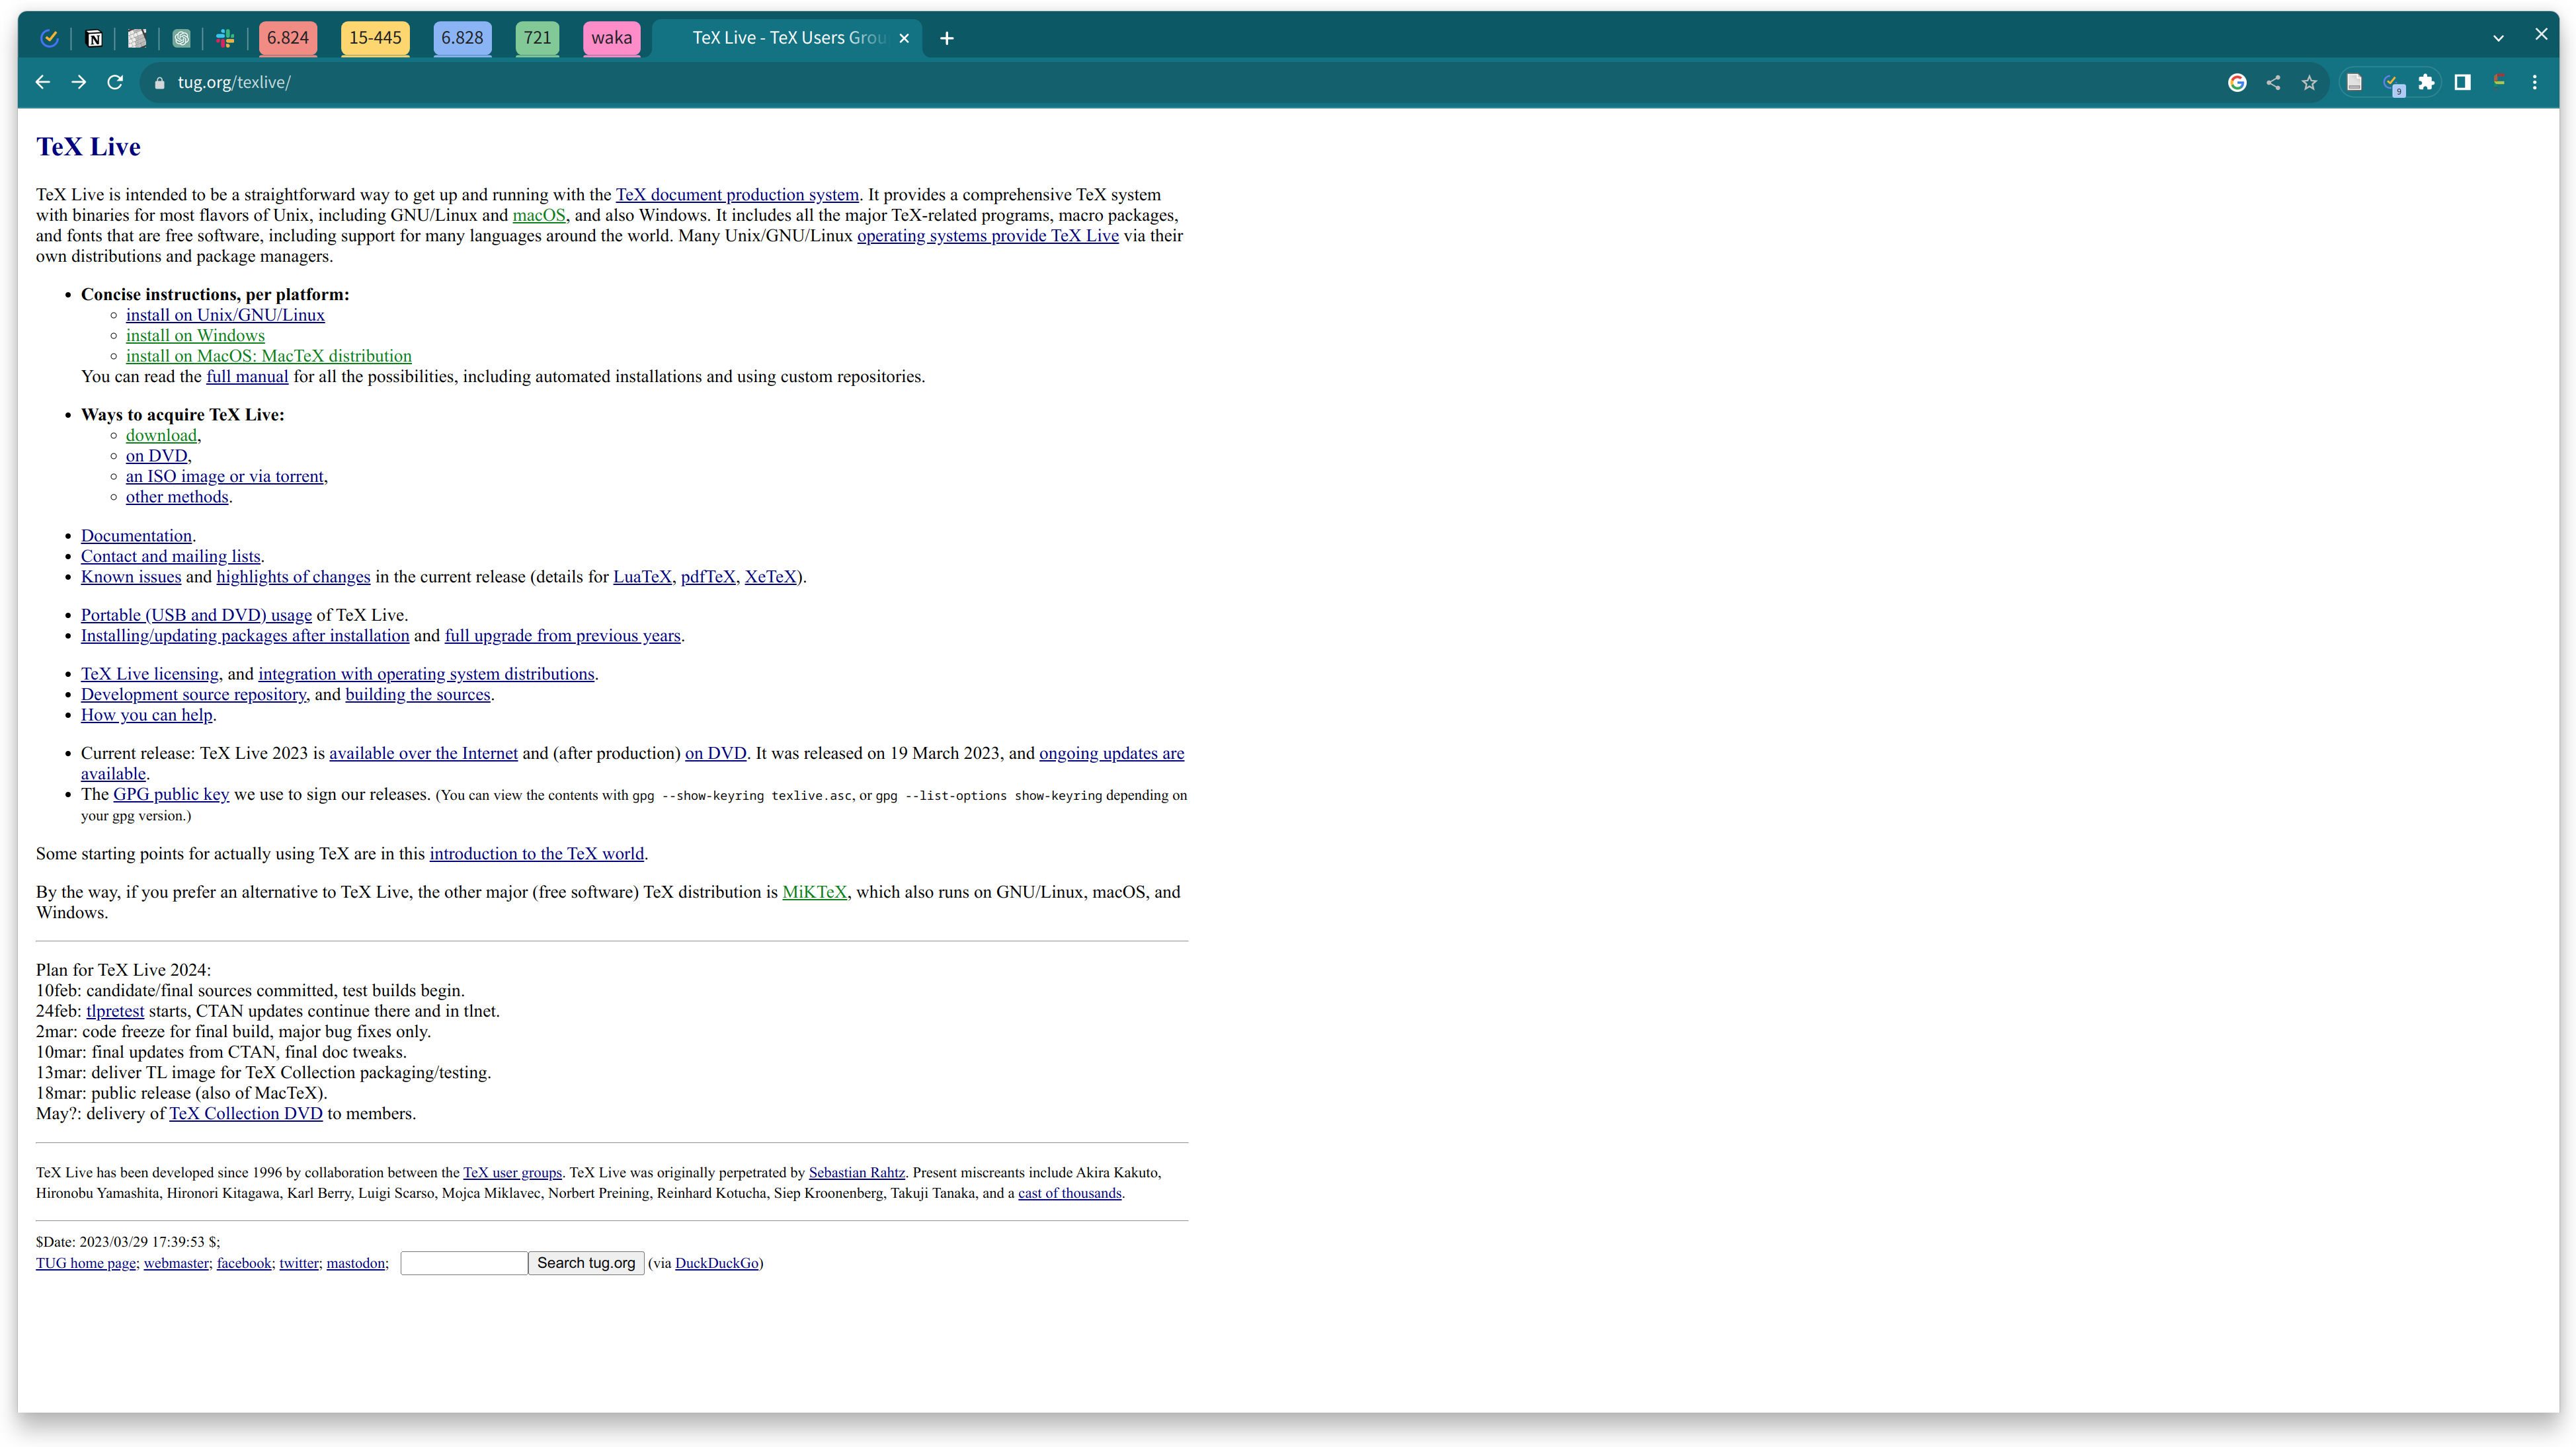
\includegraphics[width=0.85\textwidth]{imgs/local-texlive-download.png}
  \end{center}
  \caption{TeX Live 下载页面}
  \label{fig:local-texlive-download}
\end{figure}

\subsection{安装编辑器——TeXstudio}

访问 \url{https://www.texstudio.org/},下载并安装 TeXstudio。TeXstudio 是一个开源的、跨平台的、功能强大的 \LaTeX 编辑器。使用它,你可以更方便地进行 \LaTeX 的写作与编辑。

\begin{figure}[H]
  \begin{center}
    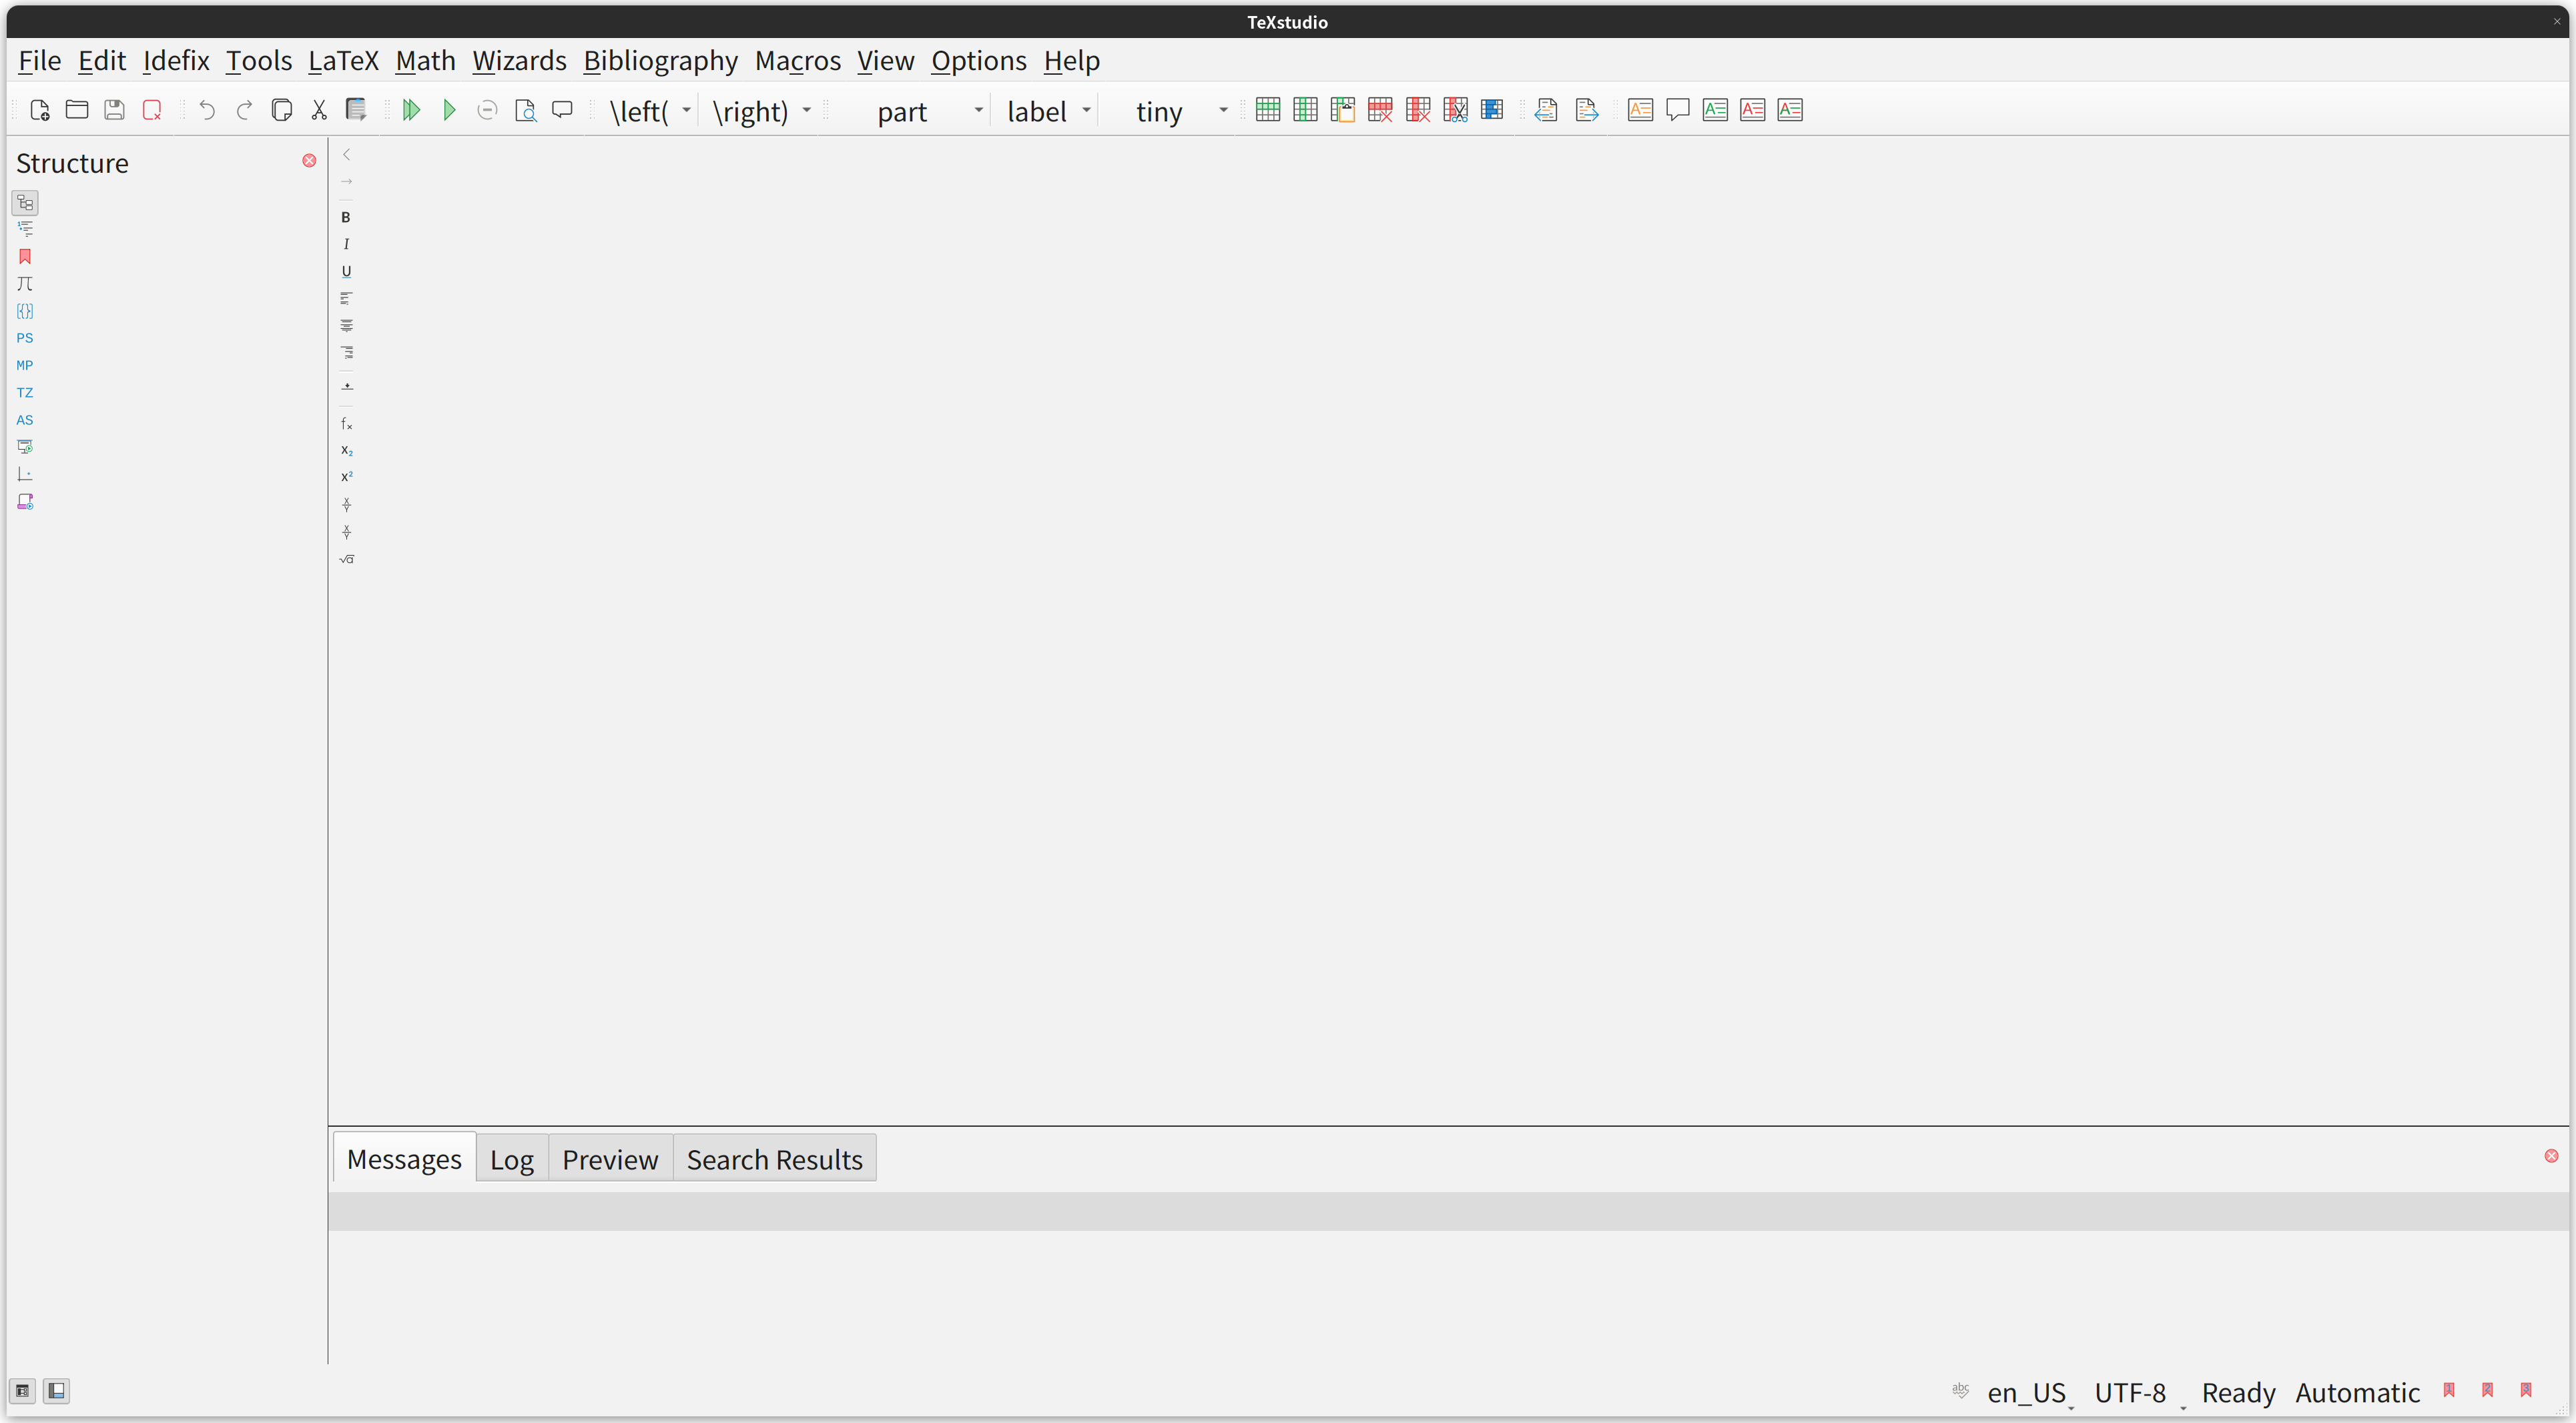
\includegraphics[width=0.85\textwidth]{imgs/texstudio-overview.png}
  \end{center}
  \caption{TeXstudio 界面}
  \label{fig:texstudio-overview}
\end{figure}

\subsection{下载模板}

\textit{如果你选择使用目前版本的模板,可以跳过该步骤。}

访问 \url{https://bithesis.bitnp.net},点击右上角的 ``模板下载'' ,跳转到 \BIThesis 项目的 GitHub Releases 页面(也即 \url{https://github.com/BITNP/BIThesis/releases/latest})。选择``graduate-thesis.zip''的模板压缩包并下载。

\begin{figure}[H]
  \begin{center}
    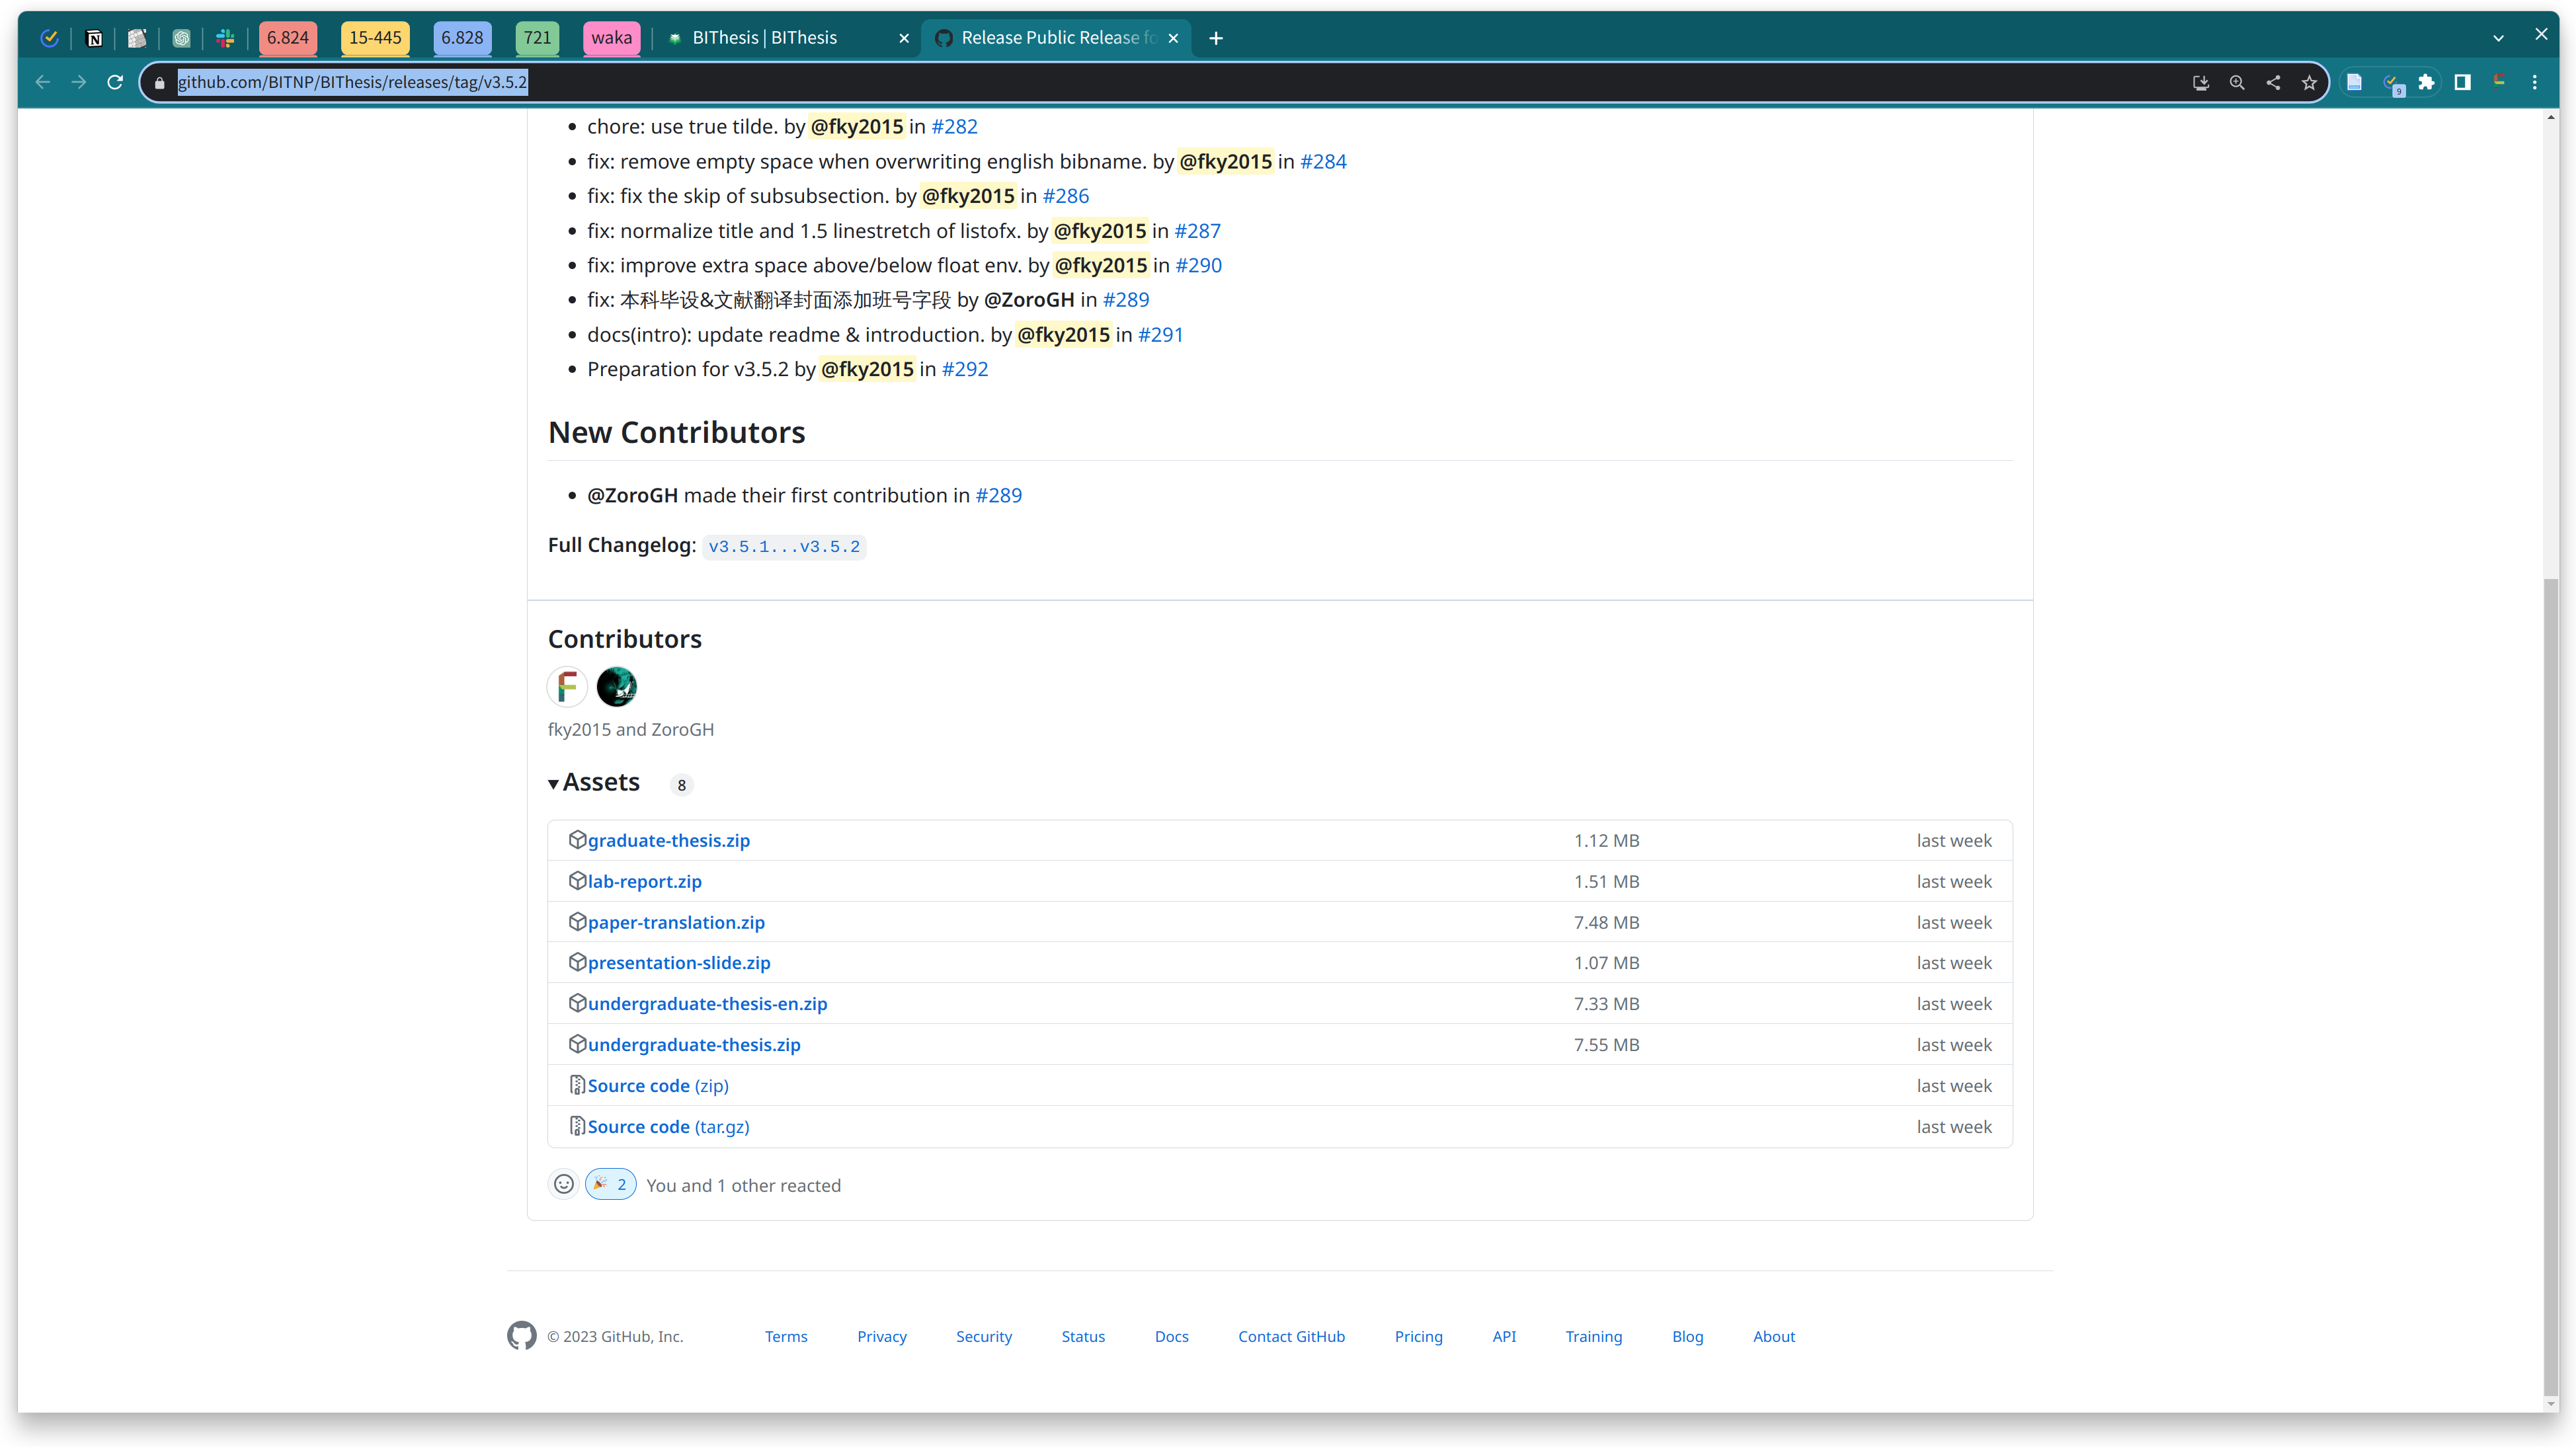
\includegraphics[width=0.85\textwidth]{imgs/github-releases.png}
  \end{center}
  \caption{模板下载页面}
  \label{fig:local-template-download}
\end{figure}

\subsection{编译生成 PDF}

解压模板压缩包,打开 TeXstudio,点击 ``File > Open'' 按钮,选择 ``main.tex'' 文件,即可打开模板。

接着,点击 ``Build \& View'' 按钮(两个叠加的绿色三角),即可编译生成 PDF。

\begin{figure}[H]
  \begin{center}
    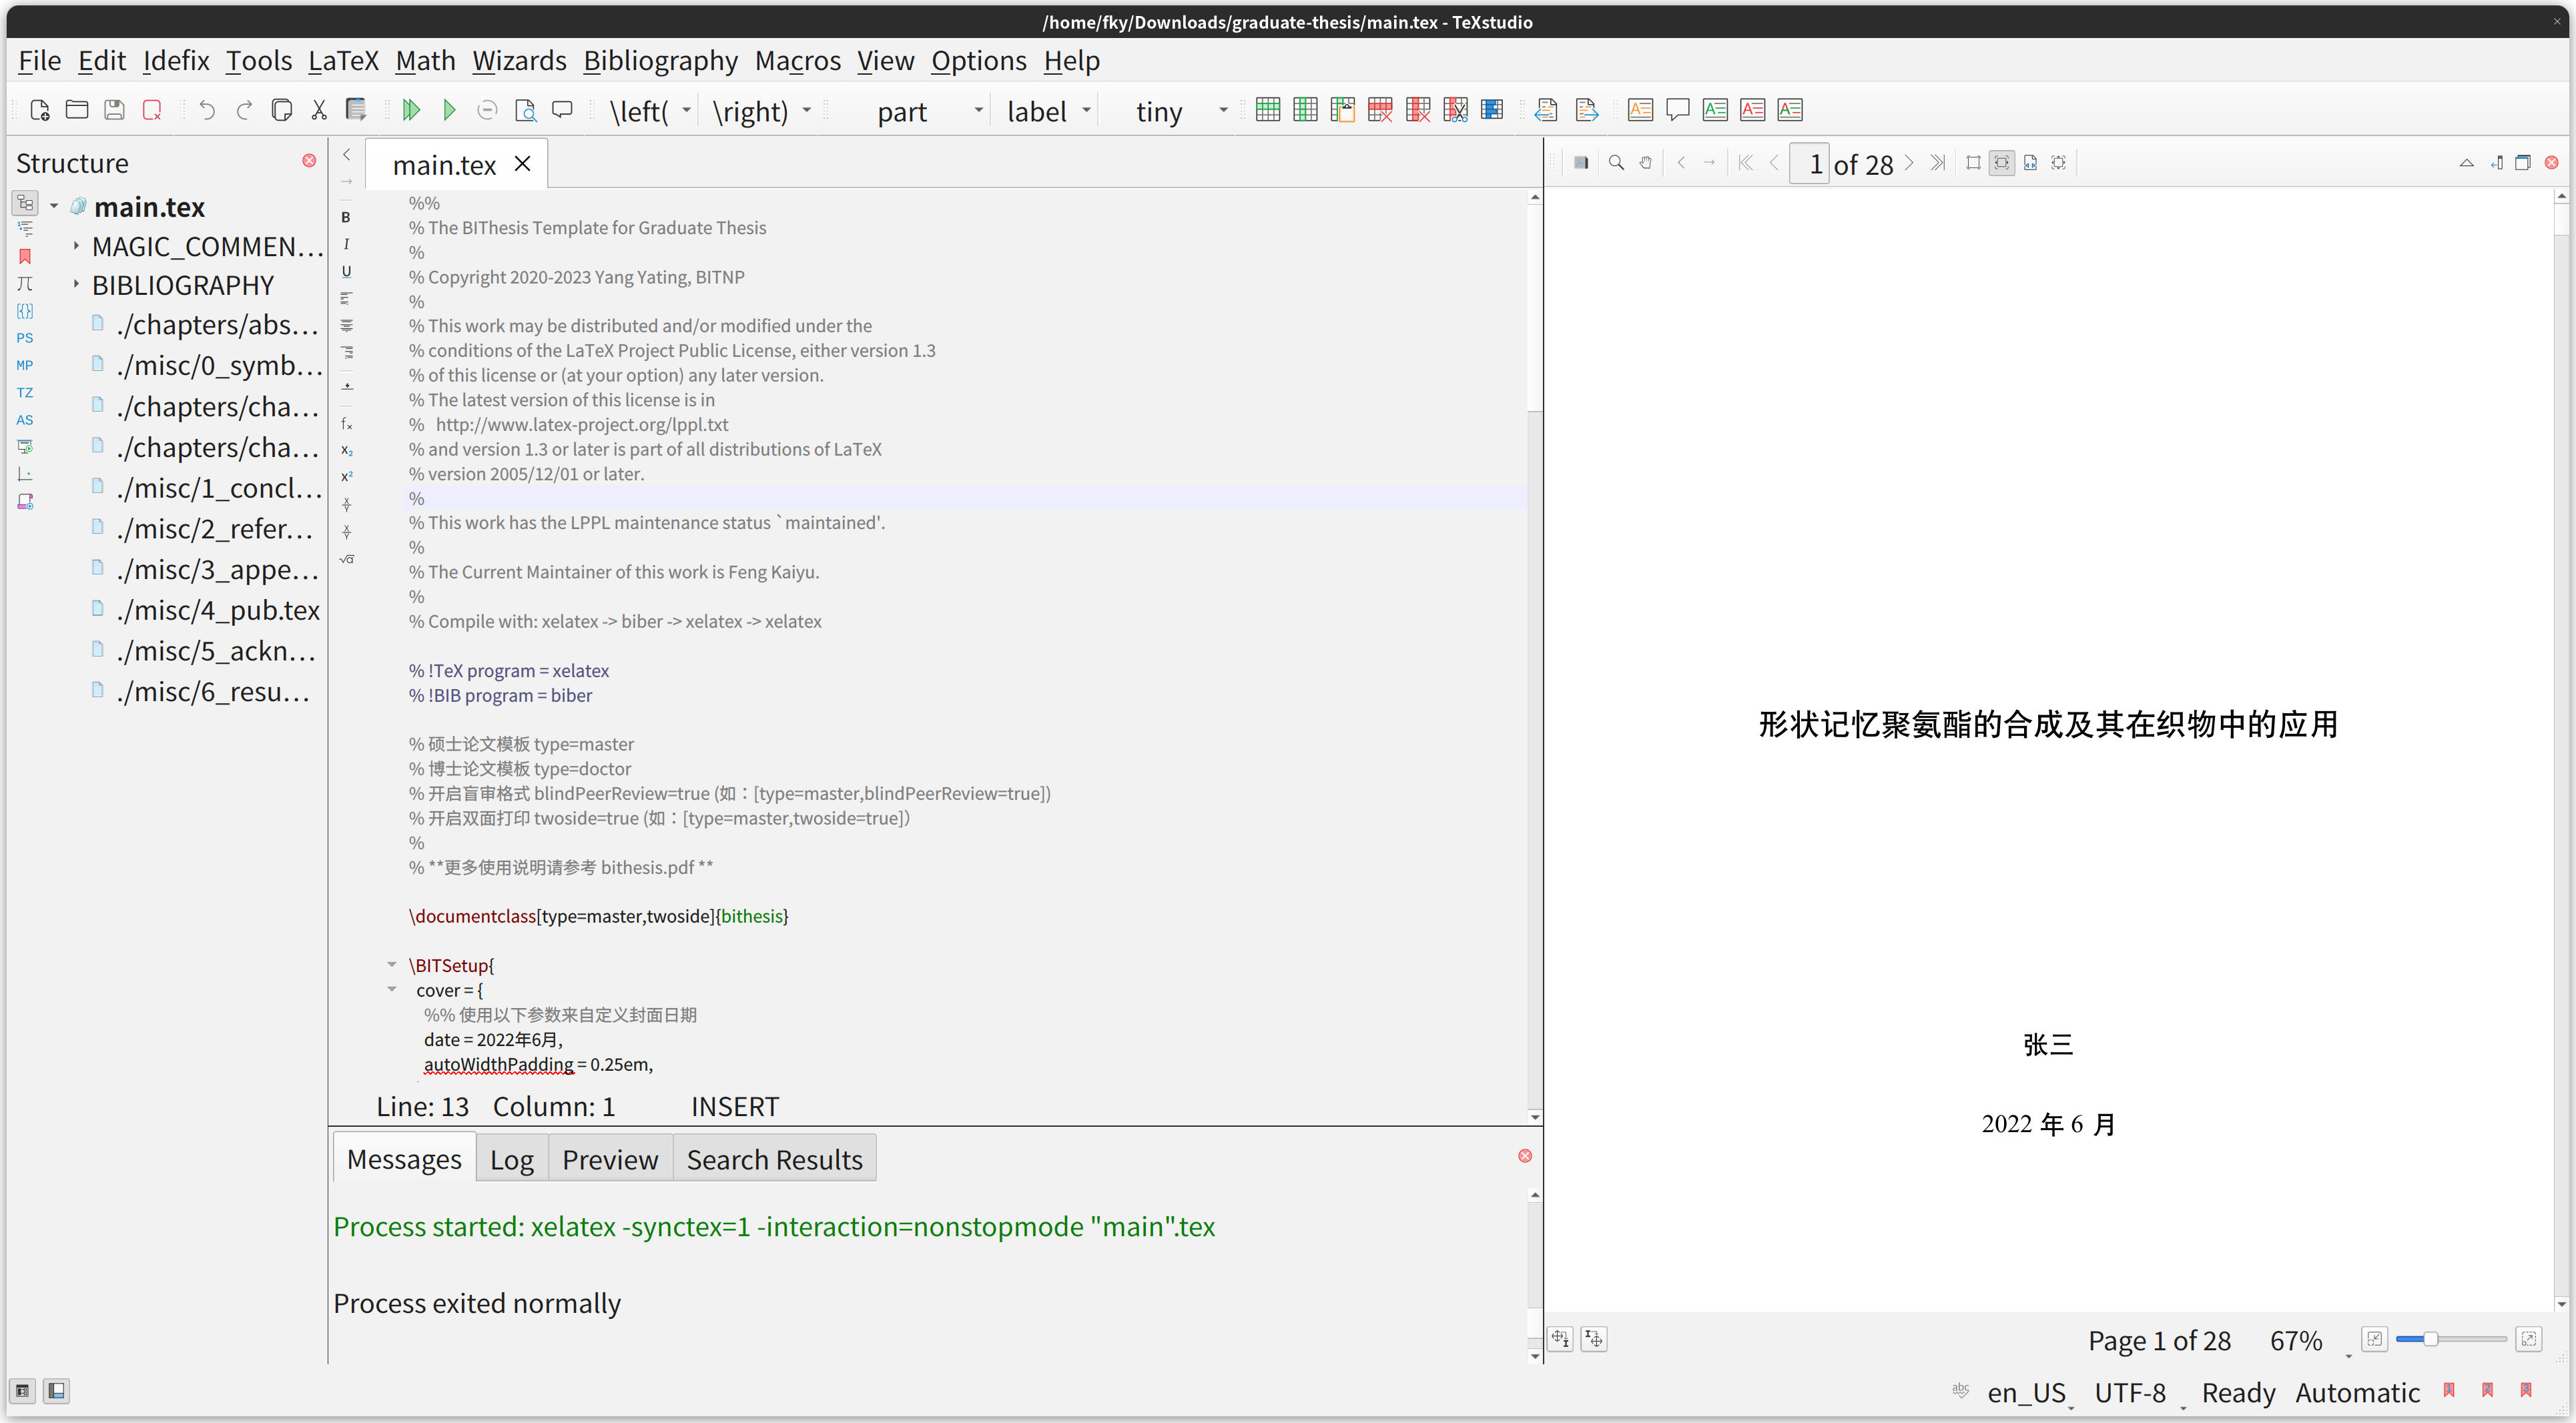
\includegraphics[width=0.85\textwidth]{imgs/texstudio-compile-and-view.png}
  \end{center}
  \caption{TeXstudio 编译生成 PDF}
  \label{fig:texstudio-compile-and-view}
\end{figure}

\section{方法二:在 Overleaf(浏览器)上编译生成 PDF}
\label{sec:overleaf-compile}

\BIThesis 项目已经在 Overleaf 上分享了多个模板,它们
会与最新版本保持同步\footnote{需要注意,你复制的模板不会自动更新。}。
因此,你可以直接在 Overleaf 上复制并使用这些模板。

\subsection{注册 Overleaf 账号}

访问 \url{https://overleaf.com}(如图\ref{fig:overleaf-register}所示),点击右上角的 ``Register'' 按钮,注册账号并登录。

\begin{figure}[H]
  \begin{center}
    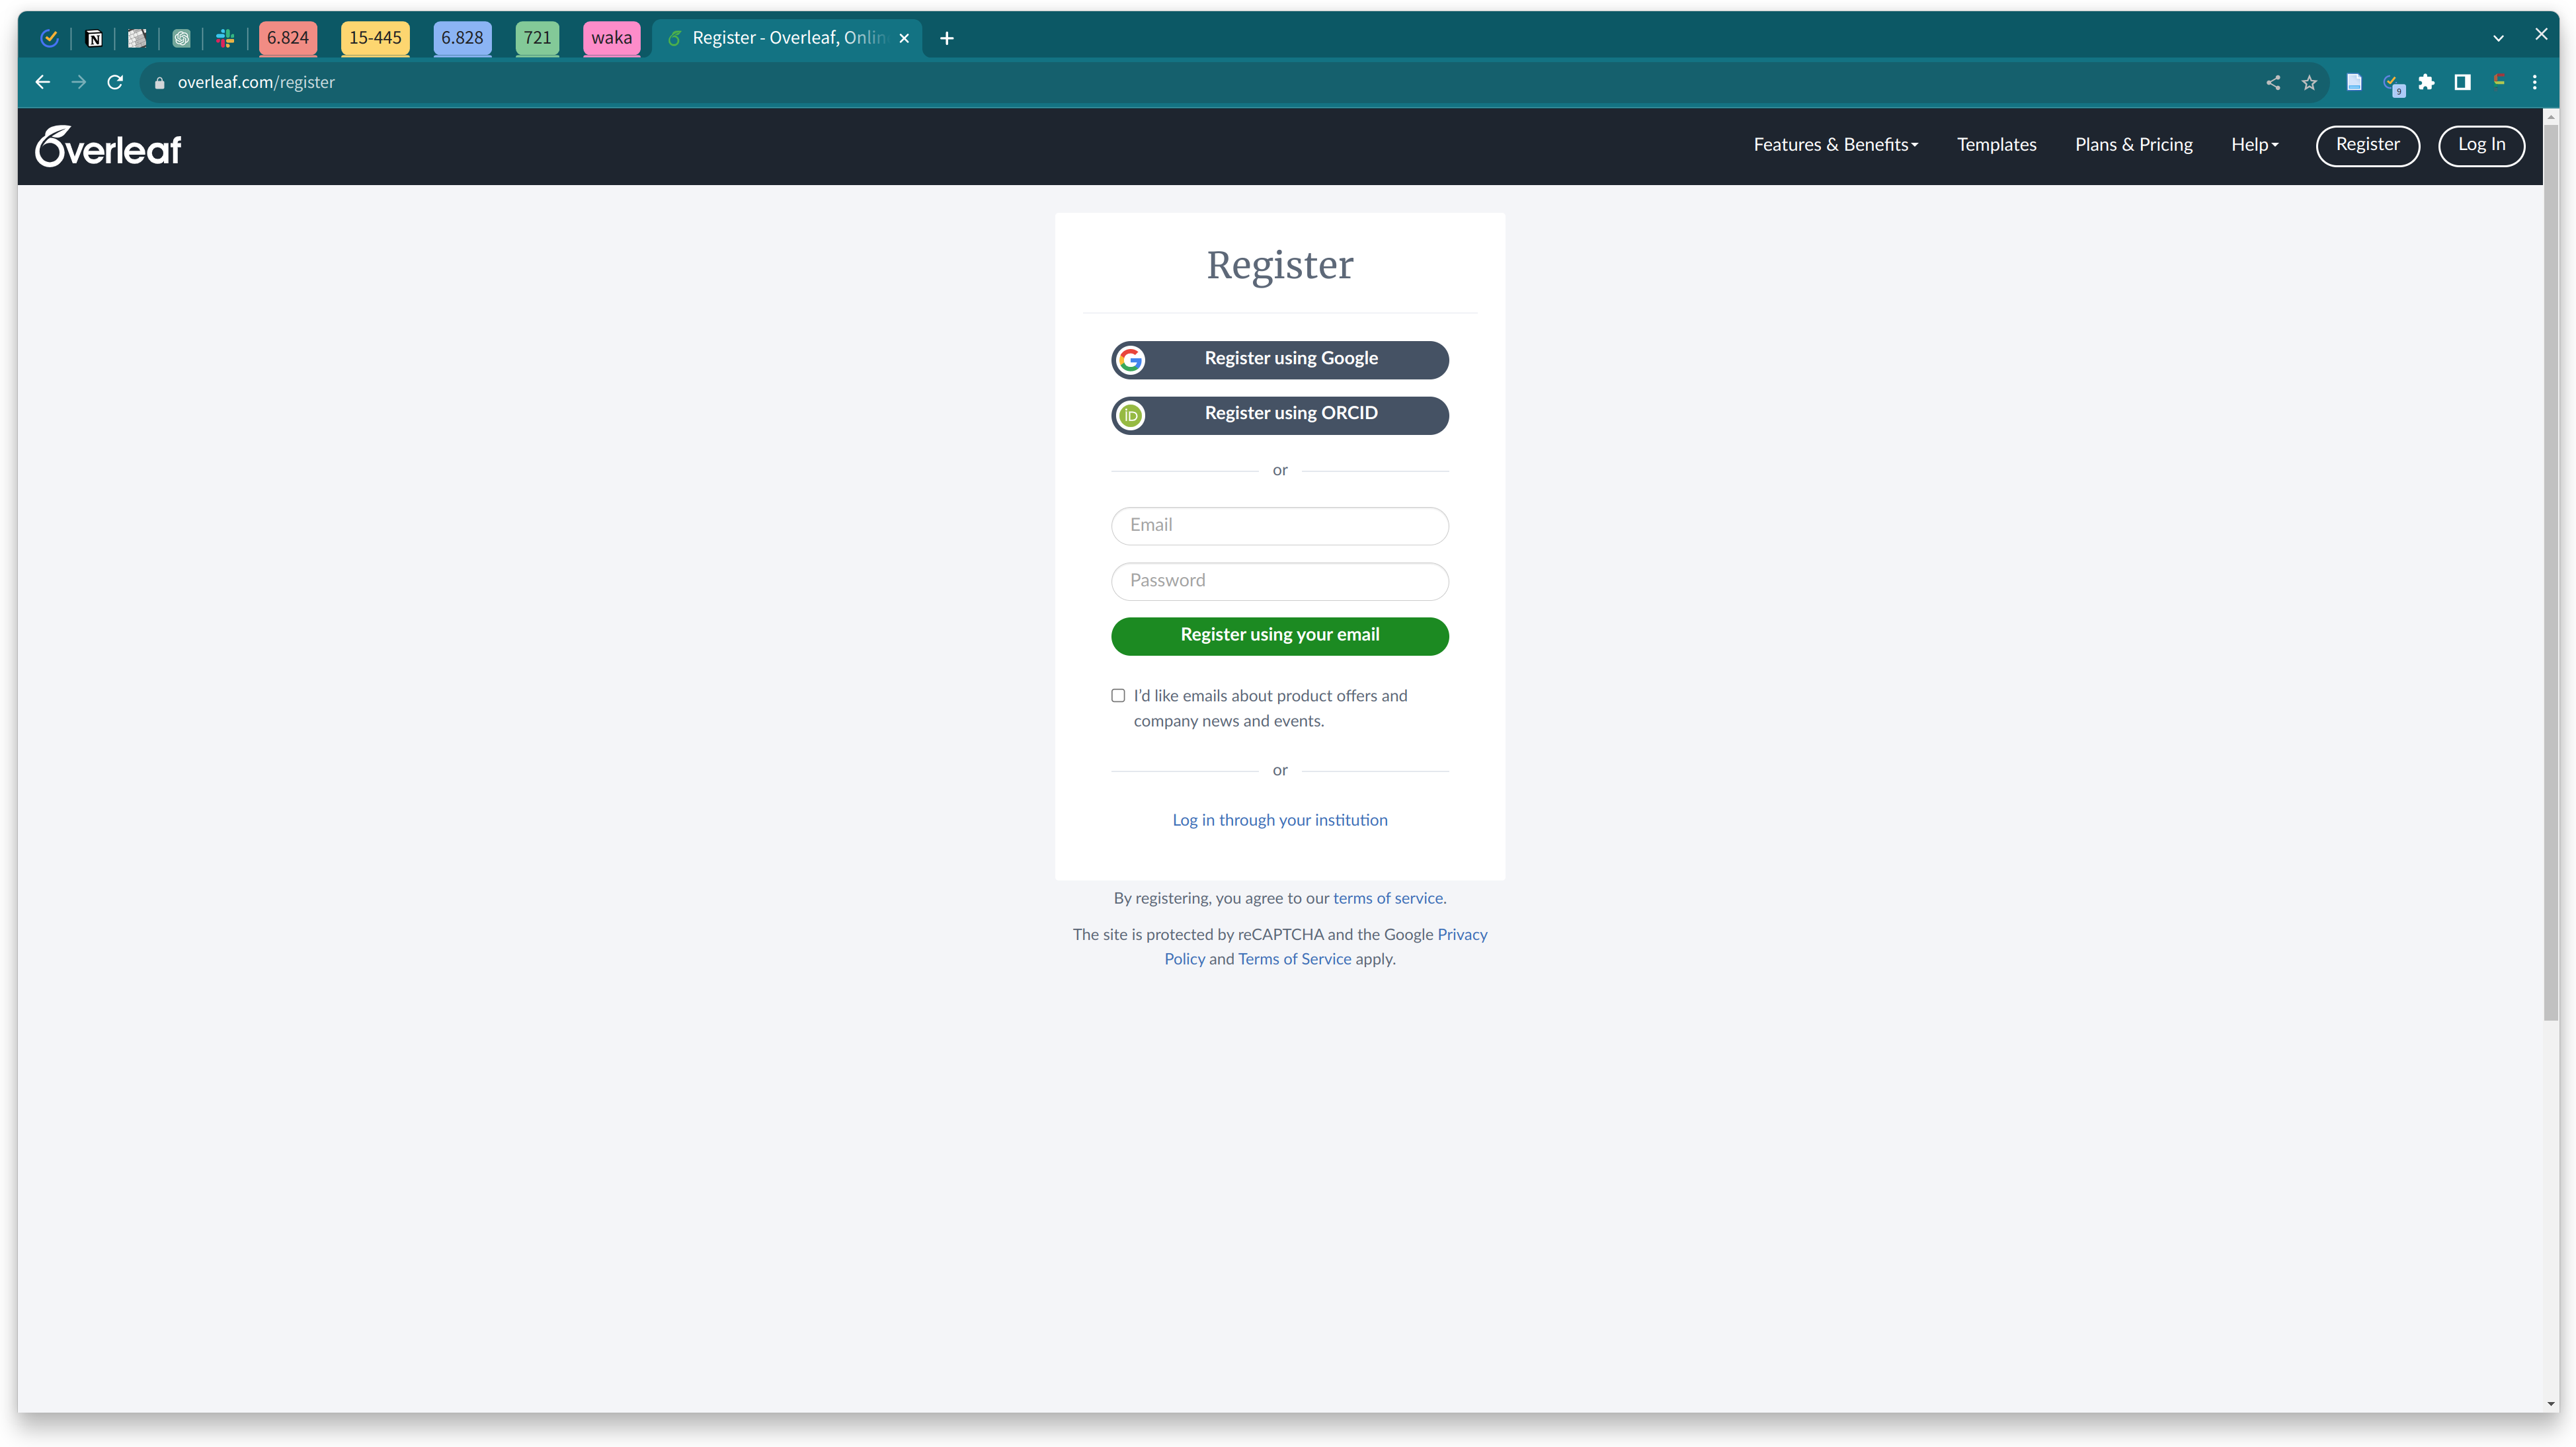
\includegraphics[width=0.85\textwidth]{imgs/overleaf-register.png}
  \end{center}
  \caption{Overleaf 注册页面}
  \label{fig:overleaf-register}
\end{figure}


\subsection{访问 \BIThesis 的 Overleaf 模板}

访问 \url{https://bithesis.bitnp.net},点击右上角的 ``Overleaf'' ,即可跳转到模板页面。

选择``研究生学位论文模板'' 模板,点击 ``Open in Overleaf'' 按钮,即可跳转到 Overleaf 上分享的项目中。

\begin{figure}[H]
  \begin{center}
    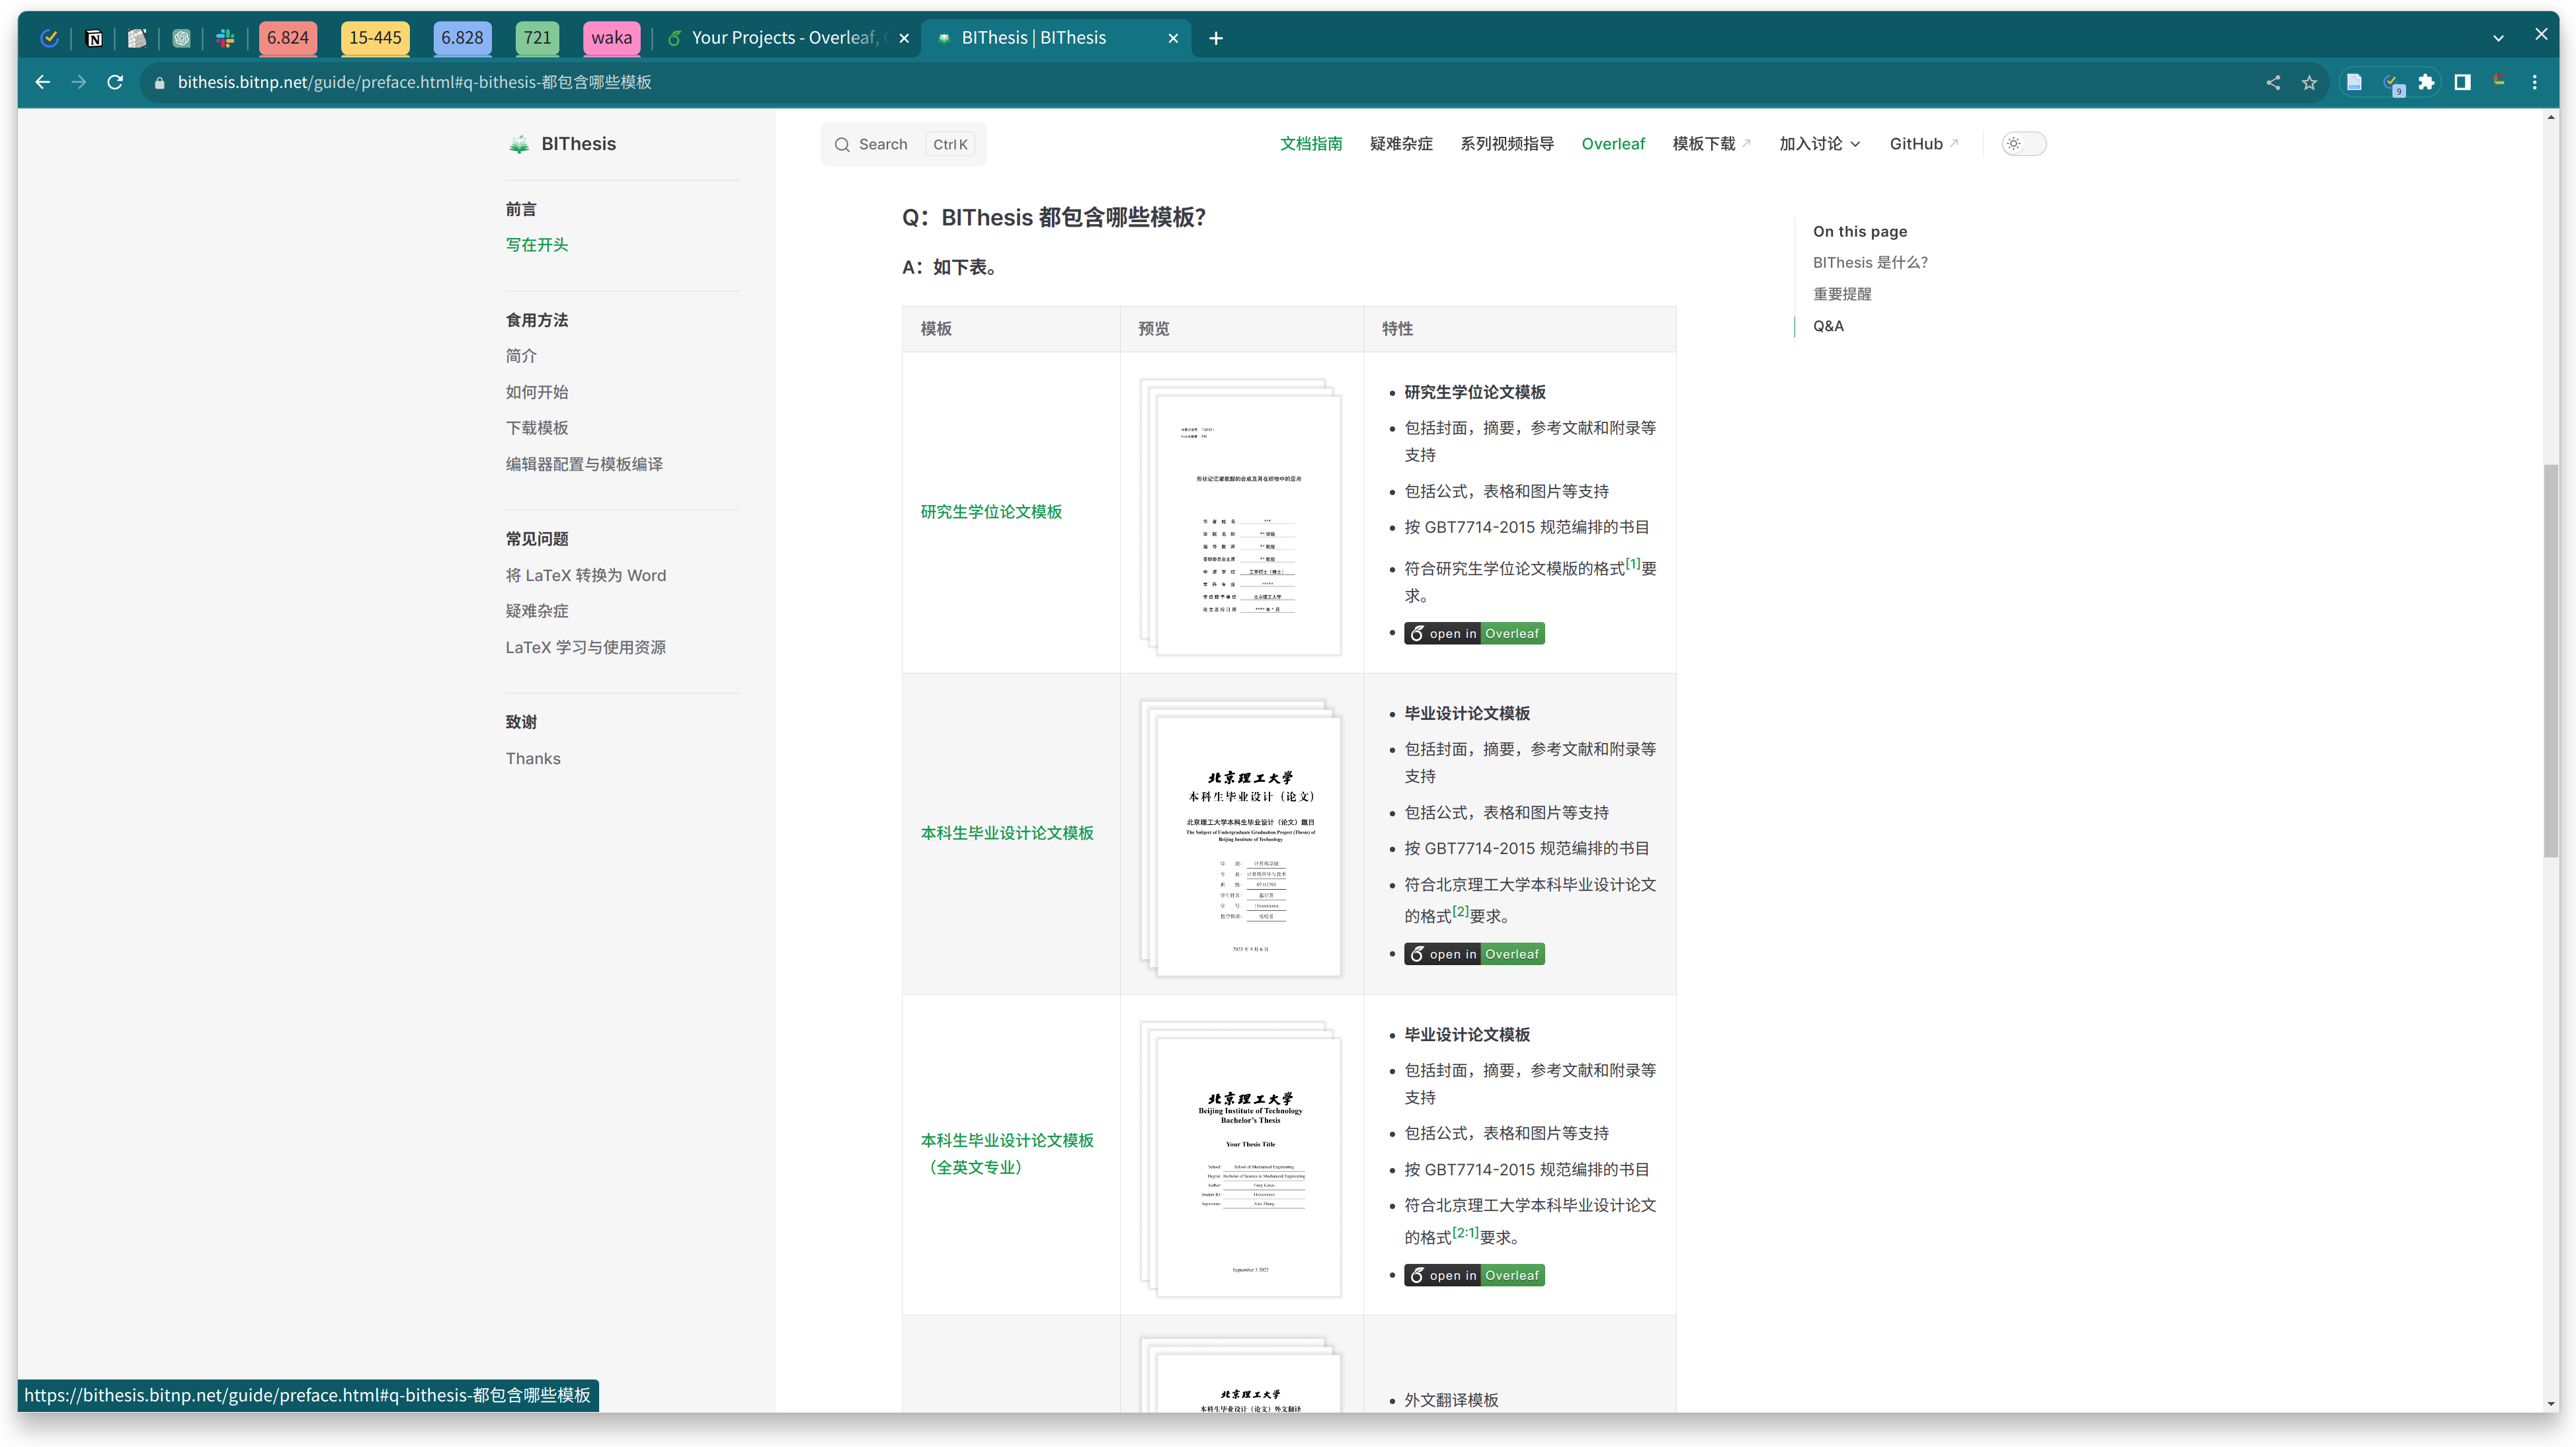
\includegraphics[width=0.85\textwidth]{imgs/overleaf-choose-template.png}
  \end{center}
  \caption{在 BIThesis-wiki 中,选择合适的模板并跳转}
  \label{fig:overleaf-template}
\end{figure}

\subsection{复制模板到自己的新项目中}

点击左上角的 ``Menu'' 按钮,选择 ``Copy Project'',即可复制模板到自己的新项目中。

\begin{figure}[H]
  \begin{center}
    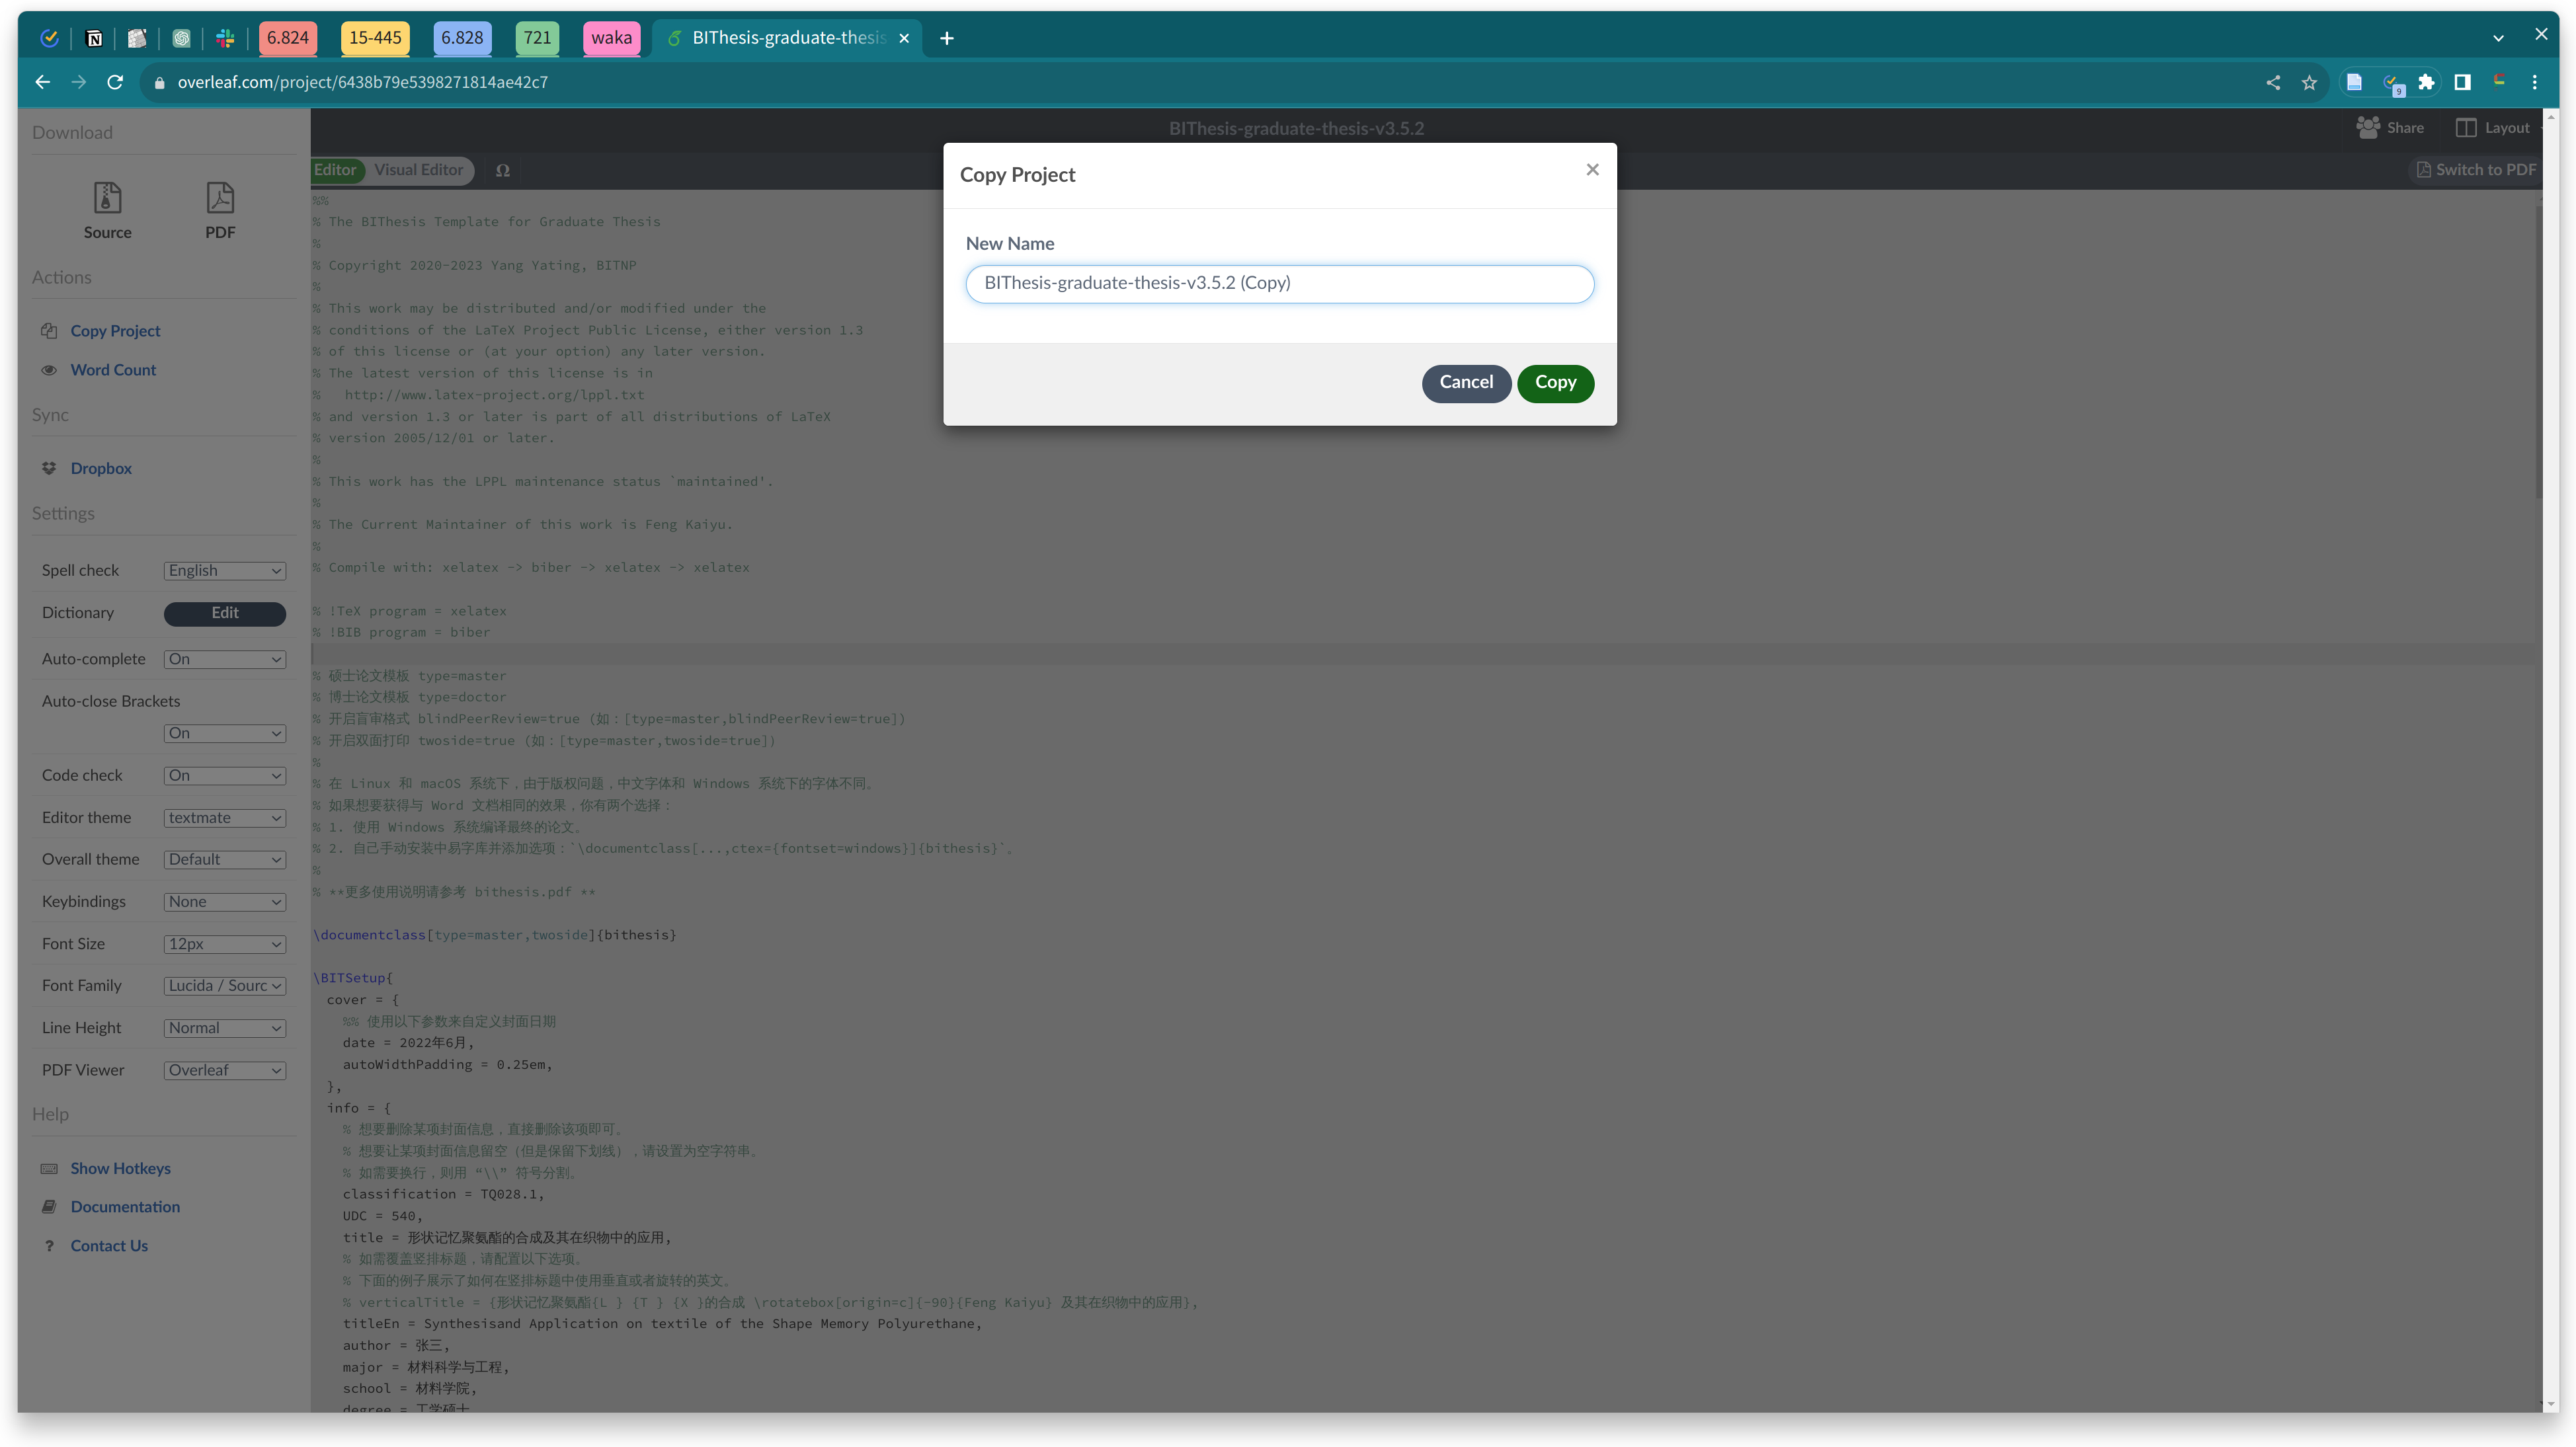
\includegraphics[width=0.85\textwidth]{imgs/overleaf-copy-project.png}
  \end{center}
  \caption{复制模板到自己的新项目中}
  \label{fig:overleaf-copy-project}
\end{figure}

\subsection{编译生成 PDF}

点击 ``Recompile'' 按钮,即可编译生成 PDF。

\begin{figure}[H]
  \begin{center}
    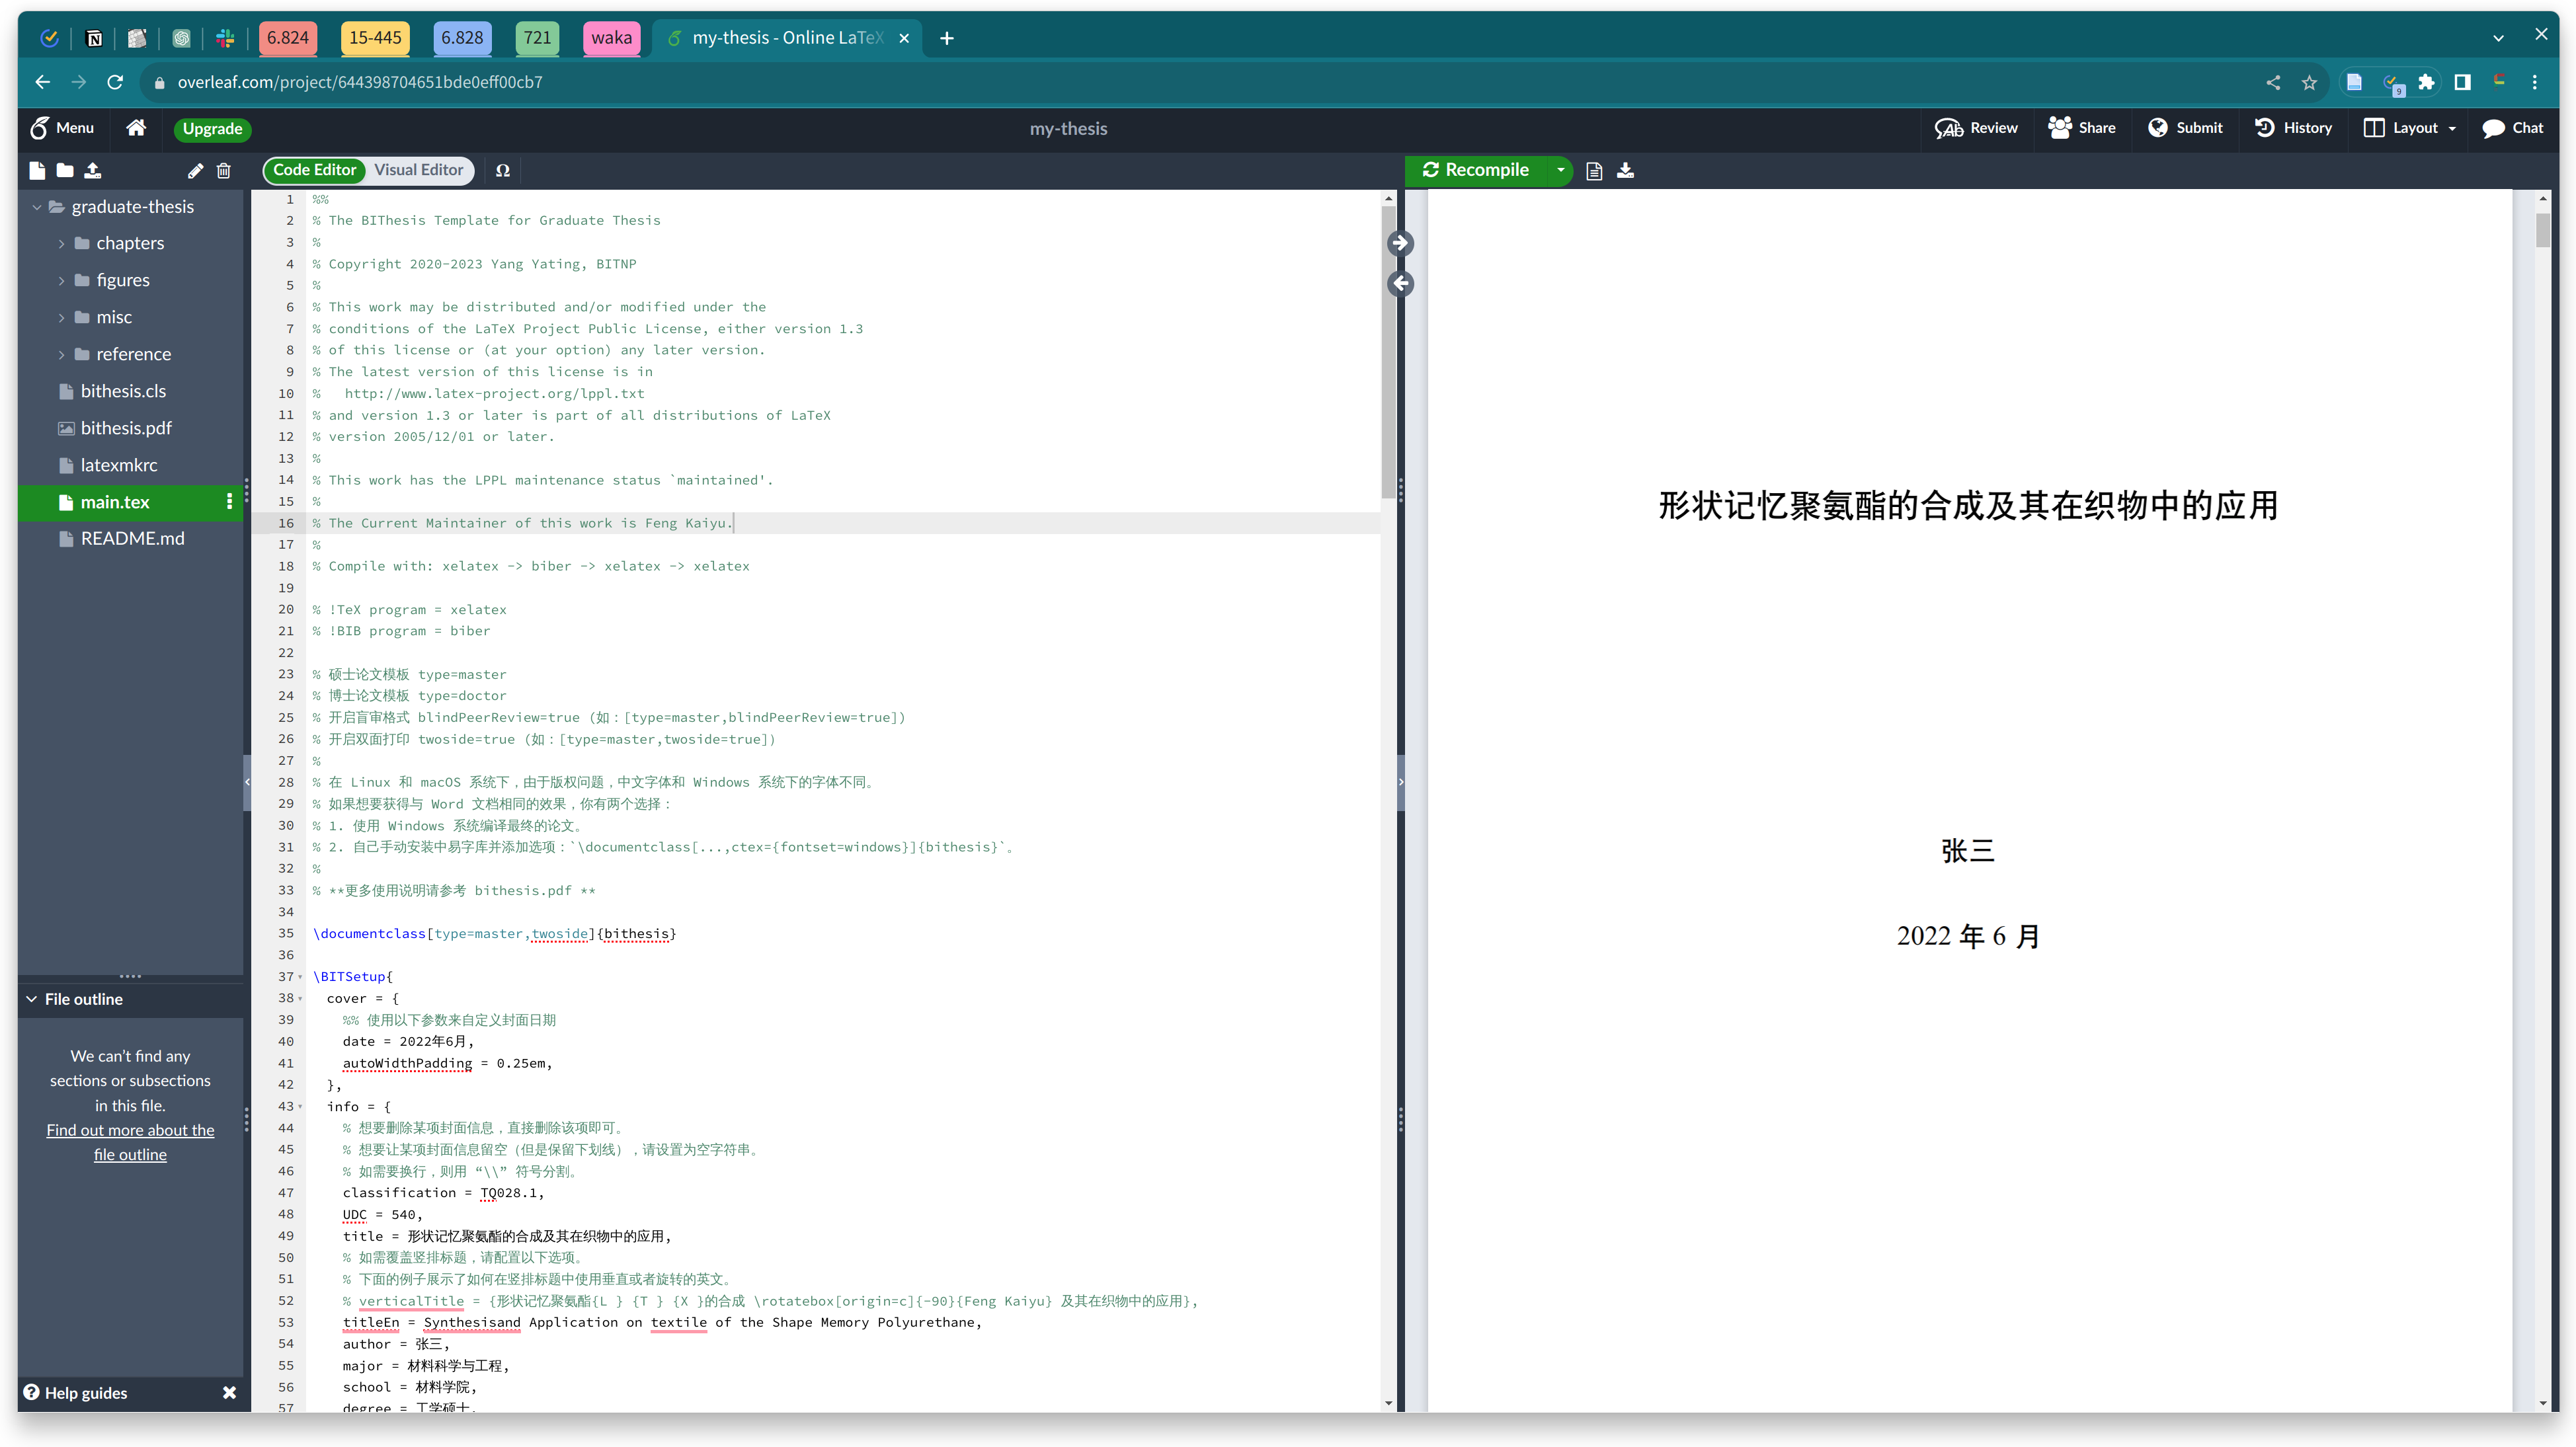
\includegraphics[width=0.85\textwidth]{imgs/overleaf-compile.png}
  \end{center}
  \caption{编译生成 PDF}
  \label{fig:overleaf-recompile}
\end{figure}


\chapter{关于 \LaTeX 和 \BIThesis 的一些疑难解答}
\label{chap:what}

\section{为什么要用 \LaTeX{} 和 \BIThesis{}?}

学术、学位论文有严格的格式要求。为了更多同学的方便使用,校方一般提供大家更为熟悉
的 Word 模板。虽然 Word 确实是大家最常用的排版工具,但是:
\begin{center}
  \kaishu
  如果你有足够多使用 Word 的经历,一定会体验过「同一份 Word 文档,在不同地方打开
  就变得不同」这样的魔幻现实主义色彩的经历。
\end{center}

\LaTeX{} 是专用于高质量的学术论文排版的排版工具,能让同学们更专注于内容本身,更
自信地排版符合格式要求的学术、学位论文。\BIThesis{} 项目旨在提供一套开箱即用的、
符合北京理工大学硕士(博士)学位论文的\LaTeX{} 模板,以助力高质量的学术写作。通
过 \BIThesis{} 模板,学生可以轻松撰写符合学校格式要求的学位论文,可避免繁琐的论
文格式调整,从而将关注点更多地放在高质量的内容本身。

\section{为何需要这么多步骤,我该如何开始?}

首先,\LaTeX{} 并不是像 Word 一样的一个开箱即用的软件。\LaTeX{} 本质上是一门用于
排版的「语言」或「语法规则」。我们实际上,是以 \underline{纯文本文件}(以
\texttt{.tex} 结尾的文件)为基础,用这样的一套 \underline{拟定好的标记语法} 来
设定文字的格式,并 \underline{利用一些工具},将其转化为符合格式要求的 PDF 文档。

我们重新回顾一下这句话:

\begin{itemize}[noitemsep]
  \item \textbf{\underline{纯文本文件}} 意味着我们只需要创建一个以 \texttt{.tex}
  结尾的文件,即可开始论文内容的撰写;
  \item \textbf{\underline{拟定好的语法}} 则需要我们了解一些 \LaTeX{} 中常用的语
  法语言规则,用来以纯文本的形式描述内容的格式,从而让下面提到的工具可以根据格式
  需要,将文档转化为PDF。
  \item \textbf{\underline{利用一些工具}} 也就表示我们需要这些工具(程序),来将
  纯文本内容转化为符合格式的 PDF 文档:我们或是下载安装他们到本地,或是使用在线
  平台开箱即用;
\end{itemize}

因此,本手册也将以这样的逻辑,为大家分别介绍每处需要的知识 --- 我们将首先介绍如
何「安装这些工具」,并如何更舒服的创建、编写此「纯文本文件」(在自己的电脑上和使
用在线的编辑器是不一样的);而后,我们将在后续的章节,简单的讲述常用的「拟定好的
语法」--- 以让大家快速上手,使用 \BIThesis{} 撰写自己的毕业论文。

\section{在自己的电脑上编写论文}

在这里,我们将在自己的电脑上配置安装撰写 \LaTeX{} 的相关工具。首先,我们搞定
\underline{一些工具} 的安装,来更方便的撰写 \underline{纯文本文件} 并将其转化为
符合格式的 PDF 文档。

\paragraph{一些工具的安装} 在 \LaTeX{} 的世界中,我们的「一些工具」包括将
\LaTeX{} 源码按照格式转换为 PDF 文档的「编译器」,和支撑部分 \LaTeX{} 格式语法的
「宏包」。我们将他们统称为一个 \LaTeX{} 发行版 --- 也就是我们需要在自己的电脑上
安装的软件。

根据同学们使用的操作系统,可以安装相应的 \LaTeX{} 发行版:

\begin{itemize}[noitemsep]
  \item \textbf{Windows 或 Linux}:下载安装 \TeX{}Live。以 Windows 为例,访问
  \href{https://www.tug.org/texlive/windows.html}{TeX Live on Windows - Easy
  install},并下载运行 \texttt{install-tl-windows.exe};
  \item \textbf{macOS}:下载安装 Mac\TeX{},即访问
  \href{https://www.tug.org/mactex/mactex-download.html}{MacTeX - Downloading
  MacTeX 2022} 并下载安装 \texttt{MacTeX.pkg};
\end{itemize}

\paragraph{纯文本文件} 我们撰写的 \LaTeX{} 文档,确实是「无格式」的纯文本文档。
也因此,任何能够编辑纯文本的工具我们其实都可以使用。但是,专业的\LaTeX{} 编辑器
一般会提供 \LaTeX{} 源码的编辑和预览功能。虽然不是必要的,但是使用编辑器可以大大
提高\LaTeX{} 的使用效率。

对于 \TeX{}Live 或者 Mac\TeX,发行版自带了基础的编辑器(分别是 \TeX{}works 和
\TeX{}Shop),可直接使用。集成的编辑环境,比如 \TeX{}studio 也是推荐大家使用的。
另外,比如 VS Code 和 Vim 等通用代码编辑器,也可以借助插件的安装,提升 \LaTeX{}
的撰写体验。

到此,我们其实就可以直接使用本模板,在自己的电脑上进行论文的编写了。如果想再了解
有关在线编辑平台 Overleaf 的相关内容,请继续阅读~\ref{sec:online-overleaf} 节;
否则,大家可以直接跳转到~\ref{sec:using-bithesis} 节,了解模板的使用方法。

\section{本地编辑或是 Overleaf 在线平台,我改使用哪一个?}
\label{sec:online-overleaf}

Overleaf 是一个在线的 \LaTeX{} 编辑器,可以直接在网页上进行 \LaTeX{} 的编辑和预
览。大家可以访问注册 \url{https://overleaf.com} 使用 Overleaf 在线编写
\LaTeX{}。选用 Overleaf 有优点也有缺点:
\begin{itemize}[noitemsep]
  \item 优点在于:
    \begin{itemize}[noitemsep]
      \item 不需要安装 \LaTeX{} 发行版,不需要配置编辑器,直接在网页上进行
      \LaTeX{} 的编辑和预览。
      \item 数据保存在云端,可以在多个设备上进行编辑和预览。
      \item 可以共享项目,方便多人协作。(对于毕业论文来说,这个优点并不是很重
      要。)
    \end{itemize}
  \item 缺点在于:
    \begin{itemize}[noitemsep]
      \item 由于 Overleaf 是一个在线的编辑器,所以需要保持网络连接,否则无法进行
      编辑和预览。
      \item 很多同学使用了第三方的文献管理软件,如 Zotero。Overleaf 无法直接与这
      些软件进行集成,需要手动导入文献。
      \item 网页版的编辑器功能有限,无法进行复杂的自定义配置。
    \end{itemize}
\end{itemize}

因此,需要使用者根据自己的需求进行选择。此外,我们的模板上传到 Overleaf 以后,需
要修改项目配置才能正常编译:
\begin{enumerate}[noitemsep]
  \item 选择左上角 \texttt{Menu} 以打开侧边栏。
  \item 修改 \texttt{Settings} 中 \texttt{Compiler} 一项的值为 \texttt{XeLaTeX}(默认为 \texttt{pdfLaTeX})。
\end{enumerate}

\chapter{模板组成与使用}
\label{sec:using-bithesis}

在本章中,我们将介绍本模板的组成部分,以及如何使用本模板和基本
的\LaTeX 语法进行论文写作。


\section{认识模板组成}

\dirtree{%
.1 /graduate-thesis/.
.2 bithesis.pdf\DTcomment{\BIThesis 模板的使用手册}. 
.2 bithesis.cls\DTcomment{模板类文件}. 
.2 latexmkrc\DTcomment{配置 latexmkrc 的编译选项}.
.2 main.tex\DTcomment{入口文件}.
.2 chapters/\DTcomment{正文内容文件夹}.
.3 abstract.tex\DTcomment{摘要}.
.3 chapter1.tex\DTcomment{章节一}.
.3 \ldots{}.
.2 figures/\DTcomment{存放了一些图片,也可以在正文写作中用于存放图片}.
.3 \ldots{}.
.2 misc/\DTcomment{包含符号表、参考文献、结论等前置、后置内容}.
.3 0\_symbols.tex.
.3 \ldots{}.
.2 references/\DTcomment{包含了「参考文献」与「成果清单」中引用的参考文献}.
.3 main.bib.
.3 pub.bib.
}

在本模板提供的文件夹中,主要包含了上方所示的几个文件夹与文件。

\subsection{模板手册 \texttt{bithesis.pdf}}

需要注意的是,\texttt{bithesis.pdf} 文件是本模板的使用手册,其中包含了
本模板的所有使用方法,以及一些注意事项。
在正式写作之前或者遇到问题时,可以先阅读该手册。

\subsection{入口文件 \texttt{main.tex}}

\texttt{main.tex} 是本模板的入口文件,其中包含了本模板的所有配置信息,
并引用了其余文件夹(\texttt{chapters/}、\texttt{figures/}、\texttt{references/})的各个章节。在这里,我们可以进行个人信息的录入,
以及通过参数调整论文的各处格式。当然,每个参数的用法都已经
在 \texttt{bithesis.pdf} 中进行了详细的说明。

\subsection{模板类文件 \texttt{bithesis.cls}}

在 \texttt{main.tex} 的最上方,我们可以看到如下的代码:
\begin{lstlisting}[language=TeX]
\documentclass[master]{bithesis}
\end{lstlisting}
这里的\texttt{bithesis}引入的就是\texttt{bithesis.cls}文件,也就是本模板的类文件。
该文件定义了本模板使用的所有格式,保证我们的论文符合学校的要求。

\subsection{主体内容文件夹}

其余的文件则一起构成了我们文章中的各个部分,其中包括了前置部分的
封面、目录、原创性声明、摘要,以及正文部分的各个章节,后置部分的
参考文献、附录、致谢等等。你可以打开这些示例文件,查看这些文件内容
都在最终的论文中起到了什么作用。得益于我们提供的模板类,我们将
大量的格式设置工作都放在你看不到的地方。而你只需要关注论文的内容——也就是
文字本身——即可。

因此我们的写作过程将变得十分简单:
\begin{enumerate}
  \item 在\texttt{main.tex}中填写个人信息,调整论文格式;
  \item 在\texttt{chapters/}文件夹中编写论文的各个章节;
  \item 补充在\texttt{misc/}、\texttt{references/}文件夹中的其他内容。
\end{enumerate}

更棒的是,我们可以通过修改配置一键生成支持盲审的论文版本——一次写作,
多种格式!

\section{个人信息录入}

在 main.tex 中,我们可以看到如下的代码:
\begin{lstlisting}[language=TeX]
\BITSetup{
  % ...
  cover = {
    %% 使用以下参数来自定义封面日期
    date = 2022年6月,
  },
  info = {
    author = 张三,
    major = 材料科学与工程,
    school = 材料学院,
    degree = 工学硕士,
    chairman = 王五教授,
    % ...
  },
  % ...
}
\end{lstlisting}

这里的各个参数就是用于控制论文封面的个人信息的。
在这里,我们用自己的信息替换掉这些默认参数,就可以生成自己的论文封面了。

上方的 cover 参数中,date 一项用于自定义封面中的日期。如果不填写该参数,
则默认使用当前的日期。

是的,就是这么简单!

有关所有参数的详细说明,可以参考 \texttt{bithesis.pdf} 中的内容。篇幅关系,不再赘述。

\section{摘要和关键字}

摘要内容,放置在 \texttt{chapters/} 文件夹中的 \texttt{abstract.tex} 文件中。
其中,摘要的关键字可在 \texttt{main.tex} 中「信息录入」的部分进行配置。

中英文摘要通过如下方式进行书写:

\begin{lstlisting}[language=TeX]
\begin{abstract}
  本文......。
\end{abstract}

\begin{abstractEn}
  In order to exploit.......
\end{abstractEn}
\end{lstlisting}


\section{论文主体}

由于已经存在了大量的示例内容、网络上已有丰富的 \LaTeX{} 的教程,
我们在这里不再赘述如何使用 \LaTeX{} 进行论文的撰写;
只是快速过一下我们在撰写论文时,使用的常用命令。

如果你对 \LaTeX{} 还不熟悉,或者想要了解更多的内容,可以参考
网络上存在的优秀的 \LaTeX{} 教程,比如 \ref{resources} 中提到的那些。

\section{其他部分}

在\texttt{misc/}文件夹中的各个文件与正文存在着下列的对应关系:
\begin{itemize}
  \item \texttt{abstract.tex} 对应着摘要;
  \item \texttt{conclusion.tex} 对应着结论;
  \item \texttt{acknowledgements.tex} 对应着致谢;
  \item \texttt{symbols.tex} 对应着符号表;
  \item \texttt{pub.bib} 对应着「攻读学位期间发表论文与研究成果清单」中的成果;
  \item \texttt{main.bib} 对应着「参考文献」中的文献。
\end{itemize}

由于在论文中,这些部分的样式固定且内容较短,因此我们
将这些部分的内容放在了单独的文件中。同时,我们也在每个
文件中提供了示例内容,以供参考。相信你在阅读这些示例内容
时,就已经知道了如何编写这些部分的内容了。

需要特殊注意的是,「成果清单」中的成果是通过引用 \texttt{pub.bib}
中的文献来生成的。因此,如果你需要在「成果清单」中添加
新的成果,那么你需要首先在 \texttt{pub.bib} 中添加新的文献条目。

而如果你想要在盲审模式中隐藏自己的名字,那么你需要
根据 pub.bib 中的示例以及注释说明,为每个文献条目添加并设置
 \texttt{author+an} 字段。
比如,如果作为张三的你的文献条目为:
\begin{lstlisting}[language=TeX]
@article{zhang2021,
  author = {张三 and 李四 and 王五},
  title = {论文标题},
  journal = {期刊名},
  year = {2021},
  volume = {1},
  pages = {1--10},
  author+an = {1:myself="\Author"},
}
\end{lstlisting}
通过设置 \texttt{author+an} 字段,我们可以在盲审模式打开时,
将自己的名字自动替换为「第一作者」。

更具体的用法,可以参考 \texttt{pub.bib} 的注释内容或者 \texttt{bithesis.pdf} 中的说明。

\subsection{交叉引用}

\subsubsection{公式和图标引用}

交叉引用的前提是需要在定义章节、公式和图表的时候都对其进行命名标签
(即\label{sec:labelName} 命令),在实际使用过程中通过标签进行引用。根据引用
的特点可以将应用分成表 \ref{tab:setSection} 中所示三类。

\begin{table}[htb]
 \centering
  \caption{章节设置关键字}     % title of Table
  \label{tab:setSection}    % label of Table
  \begin{tabular}{cl}
    \hline
    章节级别        & 关键字     \\
    \hline
     章        & \verb|\chapter| \\
     节        & \verb|\section | \\
    子节      & \verb|\subsection |\\
    表格名称       & \verb|\caption{标题名称}| \\
    引用标签       & \verb|\label{引用名称}| \\
    \hline
  \end{tabular}
\end{table}


其中,表格和图片的摆放位置由 \verb|\begin{table}| 或 \verb|\begin{figure}| 后面的中括号设
置,例如 [htb] 表示可以将图表放在当前位置(here)
、页面顶端(top)或者页面底端
(bottom)。

\subsubsection{文献引用}

\BIThesis 论文模板使用 BibLaTeX 宏包管理参考文献,使用方法与普通的 BibTeX 宏包
类似,但是更加强大。在使用时,请遵循以下步骤:
\begin{enumerate}
  \item 在 \texttt{references/main.bib} 中添加参考文献条目;
  \item 在正文中使用 \verb|\cite{key}| 或 \verb|\parencite{key}| 等命令引用文献。
\end{enumerate}



\chapter{公式、图像和表格}
\label{chap:example}

公式、图表和插图广泛使用于学位论文中,并且在正文内存在较多的交叉引用,对他们的高效处理也是\LaTeX{}的优势之一。公式、图表和插图在定义时的共同特点包含:定义中需要设定引用标签、设置图表名称。定义时,图表摆放位置并无要求,\LaTeX{}会根据文稿内容自动计算图表摆放位置,不会出现表格窜行的问题。

\section{公式与数学环境}

\subsection{公式及术语表}
\label{sec:eqn}

公式定义的内容包含在\verb|\begin{equation}|\verb|\end{equation}|之间。为方便,公式的编辑可以采用\textbf{在线的\LaTeX{}公式编辑器}(截至2023年,\href{https://www.latexlive.com/}{latexlive.com}可以视为一个不错的例子)。一般的\LaTeX{}编辑器如 TexStudio 也都会提供语法补全。

{\bf{实例1:}} 以下是L-B非稳态流动升力模型,公式引用为公式\ref{eqn:LBmodel}。该公式的术语列表见 表 \ref{tab:LB-parameters}。
\begin{equation}
 \label{eqn:LBmodel}
   C_{L}=C_{L0}+C_{L\alpha }\left ( \frac{1+\sqrt{X}}{2} \right )\alpha 
\end{equation}

\begin{lstlisting}[language={[LaTeX]TeX}, caption={L-B非稳态流动升力模型}]
\begin{equation}
 \label{eqn:LBmodel}
   C_{L}=C_{L0}+C_{L\alpha }\left ( \frac{1+\sqrt{X}}{2} \right )\alpha 
\end{equation}
\end{lstlisting}

\subsection{长公式排版}


《Math mode》里有举一个长公式排版的例子如下。《Math mode》有十分丰富实用的例子,感兴趣的同学可以参考一下。

\begin {multline}
  \frac {1}{2}\Delta (f_{ij}f^{ij})=
  2\left (\sum _{i<j}\chi _{ij}(\sigma _{i}-
    \sigma _{j}) ^{2}+ f^{ij}\nabla _{j}\nabla _{i}(\Delta f)+\right .\\
  \left .+\nabla _{k}f_{ij}\nabla ^{k}f^{ij}+
    f^{ij}f^{k}\left [2\nabla _{i}R_{jk}-
      \nabla _{k}R_{ij}\right ]\vphantom {\sum _{i<j}}\right )
\end{multline}

\begin{lstlisting}[language={[LaTeX]TeX}, caption={长公式排版}]
\begin {multline}
  \frac {1}{2}\Delta(f_{ij}f^{ij})=
  2\left(\sum_{i<j}\chi_{ij}(\sigma_{i}-
    \sigma_{j}) ^{2}+ f^{ij}\nabla_{j}\nabla_{i}(\Delta f)+\right.\\
  \left.+\nabla_{k}f_{ij}\nabla ^{k}f^{ij}+
    f^{ij}f^{k}\left [2\nabla_{i}R_{jk}-
      \nabla_{k}R_{ij}\right]\vphantom{\sum_{i<j}}\right )
\end{multline}
\end{lstlisting}

\subsection{定理环境}

在~bithesis.cls~中定义了丰富的定理\textbf{环境}
algo(算法),them(定理),lem(引理),prop(命题),cor(推论),defn(定义),conj(猜想),exmp(例),rem(注),case(情形),amsmath还提供了一个proof(证明)的环境。
这里举一个``定理''和``证明''的例子。
\begin{them}[留数定理]
\label{thm:res}
  假设$U$是复平面上的一个单连通开子集,$a_1,\ldots,a_n$是复平面上有限个点,$f$是定义在$U\backslash \{a_1,\ldots,a_n\}$上的全纯函数,
  如果$\gamma$是一条把$a_1,\ldots,a_n$包围起来的可求长曲线,但不经过任何一个$a_k$,并且其起点与终点重合,那么:

  \begin{equation}
    \label{eq:res}
    \ointop_{\gamma}f(z)\,\mathrm{d}z = 2\uppi\mathbf{i}\sum^n_{k=1}\mathrm{I}(\gamma,a_k)\mathrm{Res}(f,a_k)
  \end{equation}

  如果$\gamma$是若尔当曲线,那么$\mathrm{I}(\gamma, a_k)=1$,因此:

  \begin{equation}
    \label{eq:resthm}
    \ointop_{\gamma}f(z)\,\mathrm{d}z = 2\uppi\mathbf{i}\sum^n_{k=1}\mathrm{Res}(f,a_k)
  \end{equation}

  在这里,$\mathrm{Res}(f, a_k)$表示$f$在点$a_k$的留数,$\mathrm{I}(\gamma,a_k)$表示$\gamma$关于点$a_k$的卷绕数。
  卷绕数是一个整数,它描述了曲线$\gamma$绕过点$a_k$的次数。如果$\gamma$依逆时针方向绕着$a_k$移动,卷绕数就是一个正数,
  如果$\gamma$根本不绕过$a_k$,卷绕数就是零。

  定理\ref{thm:res}的证明。
  
  \begin{proof}
    首先,由……

    其次,……

    所以……
  \end{proof}
  
\end{them}

\begin{lstlisting}[language={[LaTeX]TeX}, caption={定理环境}]
\begin{them}[留数定理]
假设$U$是复平面上的一个单连通开子集...... 
\end{them}
\end{lstlisting}

\begin{lstlisting}[language={[LaTeX]TeX}, caption={证明环境}]
  \begin{proof}
    首先,由……
    其次,……
    所以……
  \end{proof}
\end{lstlisting}

上面的公式例子中,有一些细节需要注意。微分号d应该使用``直立体'',也就是用mathrm包围起来。
并且,微分号和被积函数之间应该有一段小间隔,可以插入\verb+\,+得到,也可使用\verb+\dif+来输入微分符号。
斜体的$d$通常只作为一般变量。
i,j作为虚数单位时,也应该使用``直立体'',为了明显,还加上了粗体,例如\verb+\mathbf{i}+。斜体$i,j$通常用作表示``序号''。
其他字母在表示常量时,也推荐使用``直立体'',譬如,圆周率$\uppi$(需要upgreek宏包),自然对数的底$\mathrm{e}$。


\section{向文档中插入图像}
\label{sec:insertimage}

\subsection{支持的图片格式}
\label{sec:imageformat}

\XeTeX~ 可以很方便地插入~PDF、EPS、PNG、JPG~格式的图片。

在学位论文中,插图地使用简单地分为两类:单列图片和多列图片。图片的格式包含*.jpg、*.eps、*.pdf,既可以是位图也可以是矢量图,在插入图片时可以定义其高度和宽度。

最基本的图片插入示例可见图\ref{fig:diagram},其代码如\ref{demo-figure1}所示。

其中\verb+\centering+表示图片居中,\verb+\includegraphics[...]{...}+导入图片并制定图片大小,\verb+\caption{}+指定图片标题,而\verb+\label{...}+为图片加上引用标签。

\begin{figure}
 \centering
 \includegraphics[width=0.75\textwidth]{example-image}
 \caption{单张图片插入的基本示例}\label{fig:diagram}
\end{figure}

\begin{lstlisting}[language={[LaTeX]TeX}, caption={示例插图代码}, label=demo-figure1]
\begin{figure}
 \centering
 \includegraphics[width=0.75\textwidth]{example-image}
 \caption{单张图片插入的基本示例}\label{fig:diagram}
\end{figure}
\end{lstlisting}

插入两幅图片的例子如\ref{fig:png-jpg}所示。
这两个水平并列放置的图共享一个``图标题''(table caption),没有各自的小标题。

\begin{figure}
  \centering
  \includegraphics[width=0.35\textwidth]{example-image-a}
  \hspace{1cm}
  \includegraphics[width=0.35\textwidth]{example-image-b}
  \caption{水平并列放置图片的基本示例}
  \label{fig:png-jpg}
\end{figure}

\begin{lstlisting}[language={[LaTeX]TeX}, caption={插入PNG/JPG}]
\begin{figure}
  \centering
  \includegraphics[width=0.35\textwidth]{example-image-a}
  \hspace{1cm}
  \includegraphics[width=0.35\textwidth]{example-image-b}
  \caption{水平并列放置图片的基本示例}
  \label{fig:png-jpg}
\end{figure}
\end{lstlisting}

更多关于~\LaTeX~ 插图的例子可以参考《~\LaTeX~插图指南》。

\subsection{长标题的换行}
\label{sec:longcaption}

图\ref{fig:longcaptionbad}和图\ref{fig:longcaptiongood}都有比较长图标题,通过对比发现,图\ref{fig:longcaptiongood}的换行效果更好一些。
其中使用了minipage环境来限制整个浮动题的宽度。

不过在实际使用中,你可以根据排版的整体效果来自行决定。

\begin{figure}
 \centering
 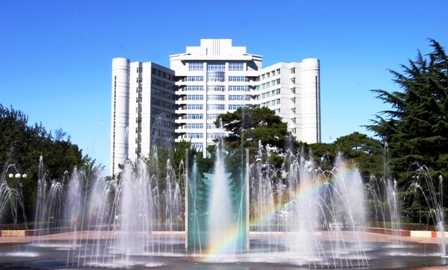
\includegraphics[width=10cm]{figures/pic1}
 \caption{BIT是我国历史最悠久的高等学府之一,是教育部直属、工信部共建的全国重点大学,985,211}
 \label{fig:longcaptionbad}
\end{figure}

\begin{figure}
  \centering
  \begin{minipage}[b]{0.6\textwidth}
  \centering
  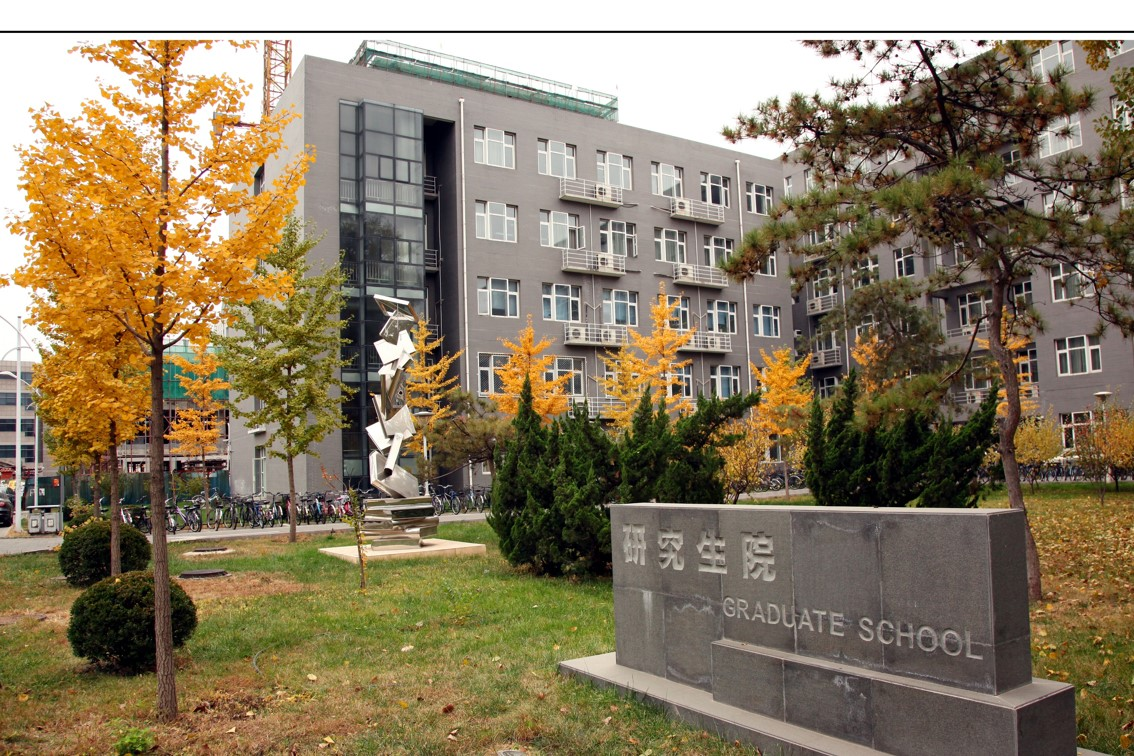
\includegraphics[width=10cm]{figures/pic2}
  \caption{BIT是我国历史最悠久的高等学府之一,是教育部直属、工信部共建的全国重点大学,985,211}
  \label{fig:longcaptiongood}
   \end{minipage}     
\end{figure}

\begin{lstlisting}[language={[LaTeX]TeX}, caption={长标题的换行}]
\begin{figure}
 \centering
 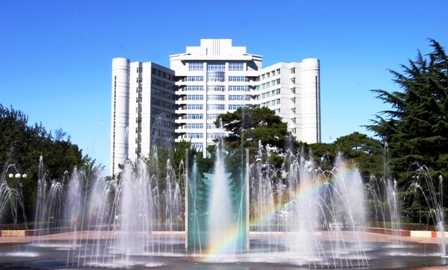
\includegraphics[width=10cm]{figures/pic1}
 \caption{BIT是我国历史最悠久的高等学府之一,是教育部直属、工信部共建的全国重点大学,985,211}
 \label{fig:longcaptionbad}
\end{figure}

\begin{figure}
  \centering
  \begin{minipage}[b]{0.6\textwidth}
  \centering
  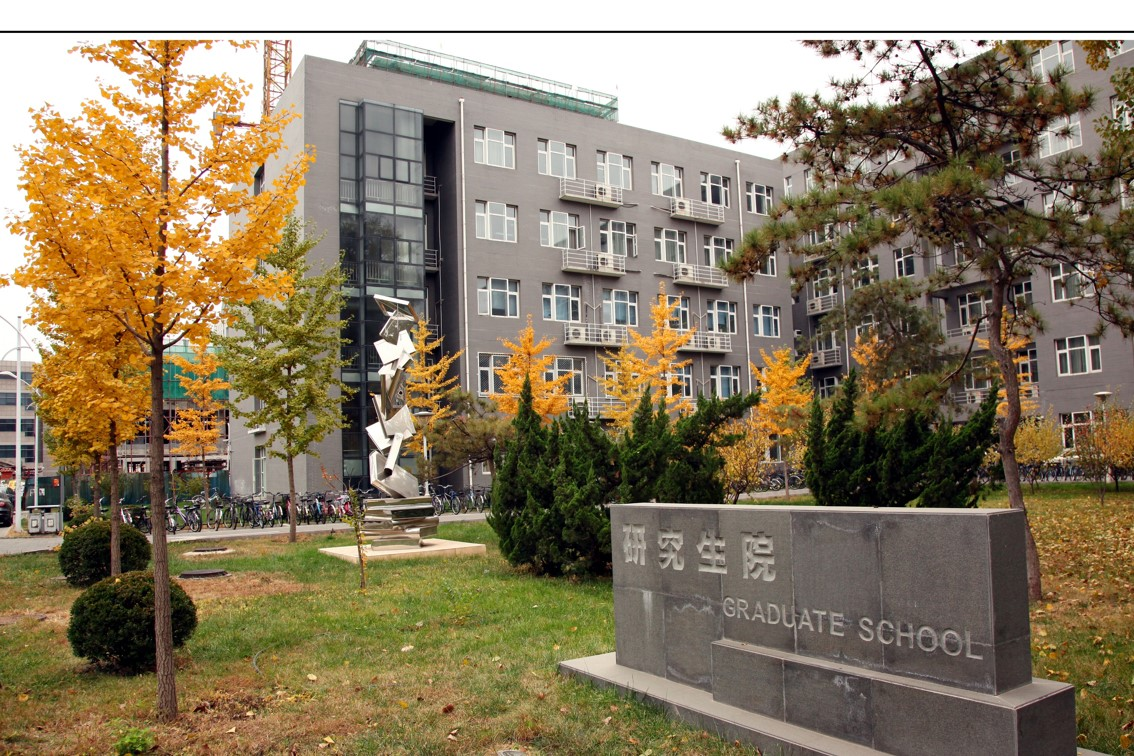
\includegraphics[width=10cm]{figures/pic2}
  \caption{BIT是我国历史最悠久的高等学府之一,是教育部直属、工信部共建的全国重点大学,985,211}
  \label{fig:longcaptiongood}
   \end{minipage}     
\end{figure}
\end{lstlisting}
  
\section{表格的例子}
\label{sec:tab}

表格的定义和引用就不多做介绍,表格内容包含在\textbackslash begin\{table\}和\textbackslash end\{table\}之间。这里给出一些表格的例子。

\textbf{\href{https://www.tablesgenerator.com/}{Tables Generator}可以用于在线生成表格}

先以模板示例中第一章的表\ref{tab:category}为例,插入代码为\ref{demo-table1}所示。

\begin{lstlisting}[language={[LaTeX]TeX}, caption={示例插表代码}, label=demo-table1]
\begin{table}
  \centering
  \caption{水系聚氨酯分类} \label{tab:category}
  \begin{tabular*}{0.9\textwidth}{@{\extracolsep{\fill}}cccc}
  \toprule
    类别			&水溶型		&胶体分散型		&乳液型 \\
  \midrule
    状态			&溶解$\sim$胶束	&分散		&白浊 \\
    外观			&水溶型		&胶体分散型		&乳液型 \\
    粒径$/\mu m$	&$<0.001$		&$0.001-0.1$		&$>0.1$ \\
    重均分子量	&$1000\sim 10000$	&数千$\sim 20万$ &$>5000$ \\
  \bottomrule
  \end{tabular*}
\end{table}
\end{lstlisting}

\begin{table}
  \centering
  \caption{模板示例中第一章的表一} \label{tab:category}
  \begin{tabular*}{0.9\textwidth}{@{\extracolsep{\fill}}cccc}
  \toprule
    类别			&水溶型		&胶体分散型		&乳液型 \\
  \midrule
    状态			&溶解$\sim$胶束	&分散		&白浊 \\
    外观			&水溶型		&胶体分散型		&乳液型 \\
    粒径$/\mu m$	&$<0.001$		&$0.001-0.1$		&$>0.1$ \\
    重均分子量	&$1000\sim 10000$	&数千$\sim 20$万 &$>5000$ \\
  \bottomrule
  \end{tabular*}
\end{table}

另举一个两列的表格例子(表\ref{tab:LB-parameters}以及代码\ref{demo-table2})。

\begin{table}              % no placement specified: defaults to here, top, bottom, page
\centering
 \begin{center}
  \caption{L-B模型中参数的物理意义}
  \label{tab:LB-parameters}
  \begin{tabular}{cl}
      \toprule
       Parameters & Physical meaning       \\
      \midrule   % \hline
       $C_{L\alpha}$ & Lift curve slope \\
       $a_{1}$ & Controls the shape of the stall curve \\
       $\alpha^{\star}$ & The break point at which $X=0.5$ \\
       $\tau_{1}$ & Represents the tendency of the model to track the static curve \\
       $\tau_{2}$ & Gives the model lift overshoot \\
      \bottomrule
  \end{tabular}
 \end{center}
\end{table}

\begin{lstlisting}[language={[LaTeX]TeX}, caption={插入表格\ref{tab:LB-parameters}}, label=demo-table2]
\begin{table}
\centering
 \begin{center}
  \caption{L-B模型中参数的物理意义}
  \begin{tabular}{cl}
      \toprule
       Parameters & Physical meaning       \\
      \midrule 
       $C_{L\alpha}$ & Lift curve slope \\
       $a_{1}$ & Controls the shape of the stall curve \\
       $\alpha^{\star}$ & The break point at which $X=0.5$ \\
       $\tau_{1}$ & Represents the tendency of the model to track the static curve \\
       $\tau_{2}$ & Gives the model lift overshoot \\
      \bottomrule
  \end{tabular}
 \end{center}
\end{table}
\end{lstlisting}

再给出一些表格的例子,如表\ref{tab:firstone}、代码\ref{demo-table3}所示。

\begin{table}
  \centering
  \caption{一个标准的三线表格}
  \label{tab:firstone}
  \begin{tabular}{@{}llr@{}} \toprule
    \multicolumn{2}{c}{Item} \\ \cmidrule(r){1-2}
    Animal & Description & Price (\$)\\ \midrule
    Gnat & per gram & 13.65 \\
    & each & 0.01 \\
    Gnu & stuffed & 92.50 \\
    Emu & stuffed & 33.33 \\
    Armadillo & frozen & 8.99 \\ \bottomrule
  \end{tabular}
\end{table}

\begin{lstlisting}[language={[LaTeX]TeX}, caption={三线表格}, label=demo-table3]
\begin{table}
  \centering
  \caption{一个标准的三线表格}
  \label{tab:firstone}
  \begin{tabular}{@{}llr@{}} \toprule
    \multicolumn{2}{c}{Item} \\ \cmidrule(r){1-2}
    Animal & Description & Price (\$)\\ \midrule
    Gnat & per gram & 13.65 \\
    & each & 0.01 \\
    Gnu & stuffed & 92.50 \\
    Emu & stuffed & 33.33 \\
    Armadillo & frozen & 8.99 \\ \bottomrule
  \end{tabular}
\end{table}
\end{lstlisting}


\section{参考文献管理}
\label{sec:reference}
\subsection{将参考文献的内容与表现分离}

\BIThesis{}论文模板使用 \href{https://www.ctan.org/pkg/biblatex}{BibLaTeX} 处理参考文献。它的出现让我们摆脱手写参考文献条目
的麻烦。
当然,使用者也可以手动编参考文献item,直接插入文档中。但是,有BibLaTeX帮助,处理起参考文献更为简单。

参考文献的具体内容就是reference文件夹下的\textit{main.bib},
参考文献的元数据(名称、作者、出处等)以一定的格式保存在这些纯文本文件中。
.bib文件也可以理解为参考文献的``数据库'',正文中所有引用的参考文件条目都会从这些文件中``析出''。
控制参考文献条目``表现形式''(格式)的代码通过 main.tex 中的 \\ \verb|\usepackage[style=gb7714-2015,...]{biblatex}| 引入。
按照学校要求,本模板使用的是国标GB/T 7714风格的参考文献析出格式(最新版本)。

.bib数据库中的参考文献条目可以手动编写,也可以在Google的学术搜索中找到。
各大数据库也支持将参考文献信息导出为.bib,省时省力。
以Google学术搜索为例:在搜索结果中,选择``引用''、``BibTeX''的连接,
点击后浏览器会打开新的标签页,出现类似代码\ref{googlescholar}所示的内容。

\begin{lstlisting}[caption={从Google Scholar找到的,但并不规范的.bib条目}, label=googlescholar, float, escapeinside="", numbers=none]
@article{张玲2000信用风险评估方法发展趋势,
  title={信用风险评估方法发展趋势},
  author={张玲 and 张佳林},
  journal={预测},
  volume={19},
  number={4},
  pages={72--75},
  year={2000}
}
\end{lstlisting}

\subsection{在正文中引用参考文献}

\textit{如果想要按照章节分别管理参考文献,可以详见 biblatex中关于refsection 的部分。简单来说,就是使用 refsection 包裹一个章节的全部内容即可。但由于我校论文要求并非采用章节管理,因此不做赘述。}

正文中引用参考文献时\cite{Jiang2005Size},用\verb+\cite{key1,key2,key3...}+可以产生“上标引用的参考文献”,
如\cite{Meta_CN,chen2007act,DPMG}。
使用\verb+\parencite{key1,key2,key3...}+则可以产生水平引用的参考文献,例如\parencite{JohnD,zhubajie,IEEE-1363}。
请看下面的例子,将会穿插使用水平的和上标的参考文献:关于书的\parencite{Meta_CN,JohnD,IEEE-1363},关于期刊的\cite{chen2007act,chen2007ewi},
会议论文\cite{DPMG,kocher99,cnproceed},
硕士学位论文\cite{zhubajie,metamori2004},博士学位论文\cite{shaheshang,FistSystem01,bai2008},标准文件\cite{IEEE-1363},技术报告\cite{NPB2},电子文献\cite{xiaoyu2001, CHRISTINE1998}。

最后总结一些注意事项:
\begin{itemize}
\item  参考文献只有在正文中被引用了,才会在最后的参考文献列表中出现;
\item  参考文献``数据库文件''.bib是纯文本文件,请使用~UTF-8~编码,不要使用~GBK~编码;
\item  参考文献条目同样有“内容”和“表现形式”之分,这种可控性是BibLaTeX带来的。
\end{itemize}


\section{用~listings~插入源代码}

这里给使用~listings~宏包插入源代码的例子,这里是一段C代码。另外,listings宏包可以实现各种复杂、漂亮的效果,想要进一步学习的同学,可以参考《The Listings Package》。

{\color{blue}
\begin{enumerate}
\item[] ~\verb|\begin{lstlisting}[language={C}, caption={一段C源代码}]|
\item[] ~\verb|#include <stdio.h>| 
\item[] ~\verb|...|
\item[] ~\verb|\end{lstlisting}|
\end{enumerate}}


\begin{lstlisting}[language={C}, caption={一段C源代码}]
#include <stdio.h>
#include <unistd.h>
#include <sys/types.h>
#include <sys/wait.h>

int main() {
  pid_t pid;

  switch ((pid = fork())) {
  case -1:
    printf("fork failed\n");
    break;
  case 0:
    /* child calls exec */
    execl("/bin/ls", "ls", "-l", (char*)0);
    printf("execl failed\n");
    break;
  default:
    /* parent uses wait to suspend execution until child finishes */
    wait((int*)0);
    printf("is completed\n");
    break;
  }

  return 0;
}
\end{lstlisting}

再给出一个插入MATLAB代码的例子。

{\color{blue}
\begin{enumerate}
\item[] ~\verb|\begin{lstlisting}[language={matlab}, caption={一段MATLAB源代码}]|
\item[] ~\verb|function paper1| 
\item[] ~\verb|r=0.05;|
\item[] ~\verb|n=100;|
\item[] ~\verb|...|
\item[] ~\verb|\end{lstlisting}|
\end{enumerate}}

\begin{lstlisting}[language={matlab}, caption={一段MATLAB源代码}]
function paper1
r=0.05;
n=100;
T=1;
X=1;
v0=0.8;
sigma=sqrt(0.08);
deltat=T/n;
for i=1:n
    t(i)=i*deltat;
    w(i)=random('norm',0,t(i),1);
end
for i=1:n
    alpha(i)=0.39;
end
for i=1:n
    temp=0;
    for k=1:i
        temp=temp+alpha(k);
    end
    B(i)=exp(r*t(i));
    BB(i)=B(i)*exp(temp*deltat);
    BBB(i)=exp(-r*(T-t(i)));
end
for i=1:n
    s0(i)=X*BBB(i);
    v(i)=v0*exp((r-0.5*sigma^2)*t(i)+sigma*w(i));
    for j=i+1:n
        D=X*BBB(j);
        d1=(log(v(i)/D)+(r+sigma^2/2)*(t(j)-t(i)))/(sigma*sqrt(t(j)-t(i)));
        d2=d1-(sigma*sqrt(t(j)-t(i)));
        ppp(i,j)=D*exp(-r*(t(j)-t(i)))*(1-cdf('normal',d2,0,1))-v(i)*(1-cdf('n
ormal',d1,0,1));
    end
end
for i=1:n
    s1(i)=0;
    for j=i+1:n
        s1(i)=s1(i)+BB(j)^(-1)*alpha(j)*deltat*(X*BBB(j)-B(j)/B(i)*ppp(i,j));
    end
    s2(i)=0;
    for j=1:n
        s2(i)=s2(i)+alpha(j);
    end
    s2(i)=X*exp(-r*T-s2(i)*deltat);
    s(i)=BB(i)*(s1(i)+s2(i));
end
plot(s)
hold on;
plot(s0);
\end{lstlisting}
  


\begin{bibprint}
  \printbibliography[heading=none,notcategory=mypub,resetnumbers=true]
\end{bibprint}

\backmatter

%%==================================================
%% conclusion.tex for BIT Master Thesis
%% modified by yang yating
%% version: 0.1
%% last update: Dec 25th, 2016
%%==================================================


\begin{conclusion}

本文采用……。{\color{blue}(结论作为学位论文正文的最后部分单独排写,但不加章号。结论是对整个论文主要结果的总结。在结论中应明确指出本研究的创新点,对其应用前景和社会、经济价值等加以预测和评价,并指出今后进一步在本研究方向进行研究工作的展望与设想。结论部分的撰写应简明扼要,突出创新性。)}

\end{conclusion}

\begin{appendices}
\label{resources}
  \chapter{学习资料}

  \section{\LaTeX 学习资料推荐}
  \begin{itemize}[nosep]
    \item \href{https://www.overleaf.com/learn/latex/Tutorials}{《Overleaf 在线文档》(英文)} 提供了非常好的在线学习资源。
    \item \href{https://texdoc.org/serve/lshort-zh-cn.pdf/0}{《一份(不太)简短的 LATEX 2ε 介绍》} 可以作为更详尽的语法手册。
  \end{itemize}

  \section{\BIThesis 模板配置使用手册}
  \BIThesis{} 使用手册位于项目文件夹的 \verb|./bithesis.pdf|。它包括了关于 \BIThesis{} 的详细使用说明,
      对于每一个配置选项都有详细的说明和示例。
      
  \chapter{\BIThesis 与北理工历代\LaTeX{}模板项目简介}
  
\begin{itemize}[nosep]
  \item 在 2017 年之前,网络上已经出现一些北京理工大学学位论文 \LaTeX 模板。
    它们是“2012大眼小蚂蚁版”和“2016汪卫版”,均以上海交通大学的模板为基础。
  \item 2017 - 2018 年,计算机学院 2016 级研究生杨雅婷等人受研究生院委托,
    制作了\href{https://github.com/BIT-thesis/LaTeX-template}{BIT-Thesis} 
    研究生学位论文模板。
  \item 2019 - 2020 年,\BIThesis 最早由 2016 级的
    武上博、王赞、唐誉铭、牟思睿和詹熠莎等人维护。
    \begin{itemize}[nosep]
    \item 此时,\BIThesis 仅支持本科生毕业论文的排版。
    \item 在此期间,\BIThesis 从无到有诞生了,包括使用手册、
      在线文档和开箱即用的模板。
    \item 同时,2017 级的赵池等同学完成了一系列 \BIThesis 
      的视频教程。
    \item 武上博推进了教务部对 \BIThesis{} 的认可工作。
  \end{itemize}
  \item 2020 - 2021 年,2017 级的冯开宇、杨思云、郝正亮和顾骁等人
      接管了维护开发工作。
  \begin{itemize}[nosep]
    \item 在此期间,冯开宇将原来的 .tex 文件制作成了宏包,并发布到 CTAN 上。
    \item 此版本是 V2 版本,代号为 Birthday Cake.
  \end{itemize}
  \item 2021 - 2022 年,2021 级(硕士研究生)的冯开宇针对 2021、
      2022 毕业季收到的反馈对该项目进行维护升级。
  \begin{itemize}[nosep]
    \item 在此期间,冯开宇合入了杨雅婷等人在 2017 年开发的研究生学位论文模板。
    \item 次年暑假期间,冯开宇用 \verb|expl3| 重构了\LaTeX 样式代码,
      向用户提供了简易易用的接口。同时,也增加了本科全英文专业的毕设论文模板样式。
    \item 此版本是 V3 版本,代号为 Summer Time.
  \end{itemize}
  \item 2023 年,冯开宇在此版本上增加了多种新的功能,并修复了一些已知的问题。
  并推进了官方(教务部、研究生院)对 \BIThesis 的认可工作。
\end{itemize}

\end{appendices}


\begin{acknowledgements}

感谢研究生院对本项目的大力支持。
特别感谢杨雅婷老师在对原有模板的大量贡献,为推动本模板官方化付出的精力。

感谢所有对本模板更新与维护做出贡献的同学和老师们,他们的名字可以在\href{https://github.com/BITNP/BIThesis/graphs/contributors}{GitHub
  Contributors} 上看到。同时, 也由衷感谢在 \href{https://github.com/BITNP/BIThesis/issues?q=}{GitHub}
对该项目上提出大量珍贵修改意见的老师和同学们。


\end{acknowledgements}


\end{document}
